% Options for packages loaded elsewhere
\PassOptionsToPackage{unicode}{hyperref}
\PassOptionsToPackage{hyphens}{url}
%
\documentclass[
]{article}
\usepackage{lmodern}
\usepackage{amssymb,amsmath}
\usepackage{ifxetex,ifluatex}
\ifnum 0\ifxetex 1\fi\ifluatex 1\fi=0 % if pdftex
  \usepackage[T1]{fontenc}
  \usepackage[utf8]{inputenc}
  \usepackage{textcomp} % provide euro and other symbols
\else % if luatex or xetex
  \usepackage{unicode-math}
  \defaultfontfeatures{Scale=MatchLowercase}
  \defaultfontfeatures[\rmfamily]{Ligatures=TeX,Scale=1}
\fi
% Use upquote if available, for straight quotes in verbatim environments
\IfFileExists{upquote.sty}{\usepackage{upquote}}{}
\IfFileExists{microtype.sty}{% use microtype if available
  \usepackage[]{microtype}
  \UseMicrotypeSet[protrusion]{basicmath} % disable protrusion for tt fonts
}{}
\makeatletter
\@ifundefined{KOMAClassName}{% if non-KOMA class
  \IfFileExists{parskip.sty}{%
    \usepackage{parskip}
  }{% else
    \setlength{\parindent}{0pt}
    \setlength{\parskip}{6pt plus 2pt minus 1pt}}
}{% if KOMA class
  \KOMAoptions{parskip=half}}
\makeatother
\usepackage{xcolor}
\IfFileExists{xurl.sty}{\usepackage{xurl}}{} % add URL line breaks if available
\IfFileExists{bookmark.sty}{\usepackage{bookmark}}{\usepackage{hyperref}}
\hypersetup{
  pdftitle={Using Census Mapper},
  pdfauthor={Simon J. Kiss},
  hidelinks,
  pdfcreator={LaTeX via pandoc}}
\urlstyle{same} % disable monospaced font for URLs
\usepackage[margin=1in]{geometry}
\usepackage{color}
\usepackage{fancyvrb}
\newcommand{\VerbBar}{|}
\newcommand{\VERB}{\Verb[commandchars=\\\{\}]}
\DefineVerbatimEnvironment{Highlighting}{Verbatim}{commandchars=\\\{\}}
% Add ',fontsize=\small' for more characters per line
\usepackage{framed}
\definecolor{shadecolor}{RGB}{248,248,248}
\newenvironment{Shaded}{\begin{snugshade}}{\end{snugshade}}
\newcommand{\AlertTok}[1]{\textcolor[rgb]{0.94,0.16,0.16}{#1}}
\newcommand{\AnnotationTok}[1]{\textcolor[rgb]{0.56,0.35,0.01}{\textbf{\textit{#1}}}}
\newcommand{\AttributeTok}[1]{\textcolor[rgb]{0.77,0.63,0.00}{#1}}
\newcommand{\BaseNTok}[1]{\textcolor[rgb]{0.00,0.00,0.81}{#1}}
\newcommand{\BuiltInTok}[1]{#1}
\newcommand{\CharTok}[1]{\textcolor[rgb]{0.31,0.60,0.02}{#1}}
\newcommand{\CommentTok}[1]{\textcolor[rgb]{0.56,0.35,0.01}{\textit{#1}}}
\newcommand{\CommentVarTok}[1]{\textcolor[rgb]{0.56,0.35,0.01}{\textbf{\textit{#1}}}}
\newcommand{\ConstantTok}[1]{\textcolor[rgb]{0.00,0.00,0.00}{#1}}
\newcommand{\ControlFlowTok}[1]{\textcolor[rgb]{0.13,0.29,0.53}{\textbf{#1}}}
\newcommand{\DataTypeTok}[1]{\textcolor[rgb]{0.13,0.29,0.53}{#1}}
\newcommand{\DecValTok}[1]{\textcolor[rgb]{0.00,0.00,0.81}{#1}}
\newcommand{\DocumentationTok}[1]{\textcolor[rgb]{0.56,0.35,0.01}{\textbf{\textit{#1}}}}
\newcommand{\ErrorTok}[1]{\textcolor[rgb]{0.64,0.00,0.00}{\textbf{#1}}}
\newcommand{\ExtensionTok}[1]{#1}
\newcommand{\FloatTok}[1]{\textcolor[rgb]{0.00,0.00,0.81}{#1}}
\newcommand{\FunctionTok}[1]{\textcolor[rgb]{0.00,0.00,0.00}{#1}}
\newcommand{\ImportTok}[1]{#1}
\newcommand{\InformationTok}[1]{\textcolor[rgb]{0.56,0.35,0.01}{\textbf{\textit{#1}}}}
\newcommand{\KeywordTok}[1]{\textcolor[rgb]{0.13,0.29,0.53}{\textbf{#1}}}
\newcommand{\NormalTok}[1]{#1}
\newcommand{\OperatorTok}[1]{\textcolor[rgb]{0.81,0.36,0.00}{\textbf{#1}}}
\newcommand{\OtherTok}[1]{\textcolor[rgb]{0.56,0.35,0.01}{#1}}
\newcommand{\PreprocessorTok}[1]{\textcolor[rgb]{0.56,0.35,0.01}{\textit{#1}}}
\newcommand{\RegionMarkerTok}[1]{#1}
\newcommand{\SpecialCharTok}[1]{\textcolor[rgb]{0.00,0.00,0.00}{#1}}
\newcommand{\SpecialStringTok}[1]{\textcolor[rgb]{0.31,0.60,0.02}{#1}}
\newcommand{\StringTok}[1]{\textcolor[rgb]{0.31,0.60,0.02}{#1}}
\newcommand{\VariableTok}[1]{\textcolor[rgb]{0.00,0.00,0.00}{#1}}
\newcommand{\VerbatimStringTok}[1]{\textcolor[rgb]{0.31,0.60,0.02}{#1}}
\newcommand{\WarningTok}[1]{\textcolor[rgb]{0.56,0.35,0.01}{\textbf{\textit{#1}}}}
\usepackage{graphicx}
\makeatletter
\def\maxwidth{\ifdim\Gin@nat@width>\linewidth\linewidth\else\Gin@nat@width\fi}
\def\maxheight{\ifdim\Gin@nat@height>\textheight\textheight\else\Gin@nat@height\fi}
\makeatother
% Scale images if necessary, so that they will not overflow the page
% margins by default, and it is still possible to overwrite the defaults
% using explicit options in \includegraphics[width, height, ...]{}
\setkeys{Gin}{width=\maxwidth,height=\maxheight,keepaspectratio}
% Set default figure placement to htbp
\makeatletter
\def\fps@figure{htbp}
\makeatother
\setlength{\emergencystretch}{3em} % prevent overfull lines
\providecommand{\tightlist}{%
  \setlength{\itemsep}{0pt}\setlength{\parskip}{0pt}}
\setcounter{secnumdepth}{-\maxdimen} % remove section numbering

\title{Using Census Mapper}
\author{Simon J. Kiss}
\date{13/03/2020}

\begin{document}
\maketitle

\hypertarget{understanding-the-hierarchical-nature-of-statistics-canada-data}{%
\section{Understanding The Hierarchical Nature of Statistics Canada
Data}\label{understanding-the-hierarchical-nature-of-statistics-canada-data}}

As I mentioned in class the other data, Statistics CAnada has a
systematic - but complex - way of categorizing its data based on
geographic areas. It is hierarchical in nature, so data is aggregated
into a variety of levels.

One way is:

\begin{verbatim}
1.(PR) Province
2. (CD) Census District (or Division, I've seen both) 
\end{verbatim}

\begin{quote}
``Group of neighbouring municipalities joined together for the purposes
of regional planning and managing common services (such as police or
ambulance services). These groupings are established under laws in
effect in certain provinces of Canada. Census division (CD) is the
general term for provincially legislated areas (such as county,
municipalité régionale de comté and regional district) or their
equivalents.'' \hfill ---
\href{https://www12.statcan.gc.ca/census-recensement/2016/ref/dict/geo008-eng.cfm}{Statistics
Canada}
\end{quote}

\begin{verbatim}
3. Census Subdivision (CSD)
     * These vary by province. In ONtario, these are cities, Indian Reserves, or municipalities (e.g. townships, I think)

4. Census Tracts (CSD)
\end{verbatim}

\begin{quote}
``Area that is small and relatively stable. Census tracts usually have a
population between 2,500 and 8,000 persons. They are located in census
metropolitan areas and in census agglomerations that have a core
population of 50,000 or more.'' \hfill ---
\href{https://www12.statcan.gc.ca/census-recensement/2011/ref/dict/geo013-eng.cfm}{Statistics
Canada}
\end{quote}

In addition, there are other categories that reflect a parallel
hierarchy. Probably the most important of these are: Census Metropolitan
Areas and Census Agglomerations.

\begin{quote}
``Area consisting of one or more neighbouring municipalities situated
around a core. A census metropolitan area must have a total population
of at least 100,000 of which 50,000 or more live in the core. A census
agglomeration must have a core population of at least 10,000.''
\hfill ---
\href{https://www12.statcan.gc.ca/census-recensement/2011/ref/dict/geo009-eng.cfm}{Statistics
Canada}
\end{quote}

\hypertarget{geographic-files-and-data-files}{%
\section{Geographic Files and Data
Files}\label{geographic-files-and-data-files}}

As well, the other thing to keep in mind is that we need to get
geography files, usually \texttt{.shp} file extension, that contain
information about each boundary and an identifier. When you look at
\texttt{.shp} files, you'll see that each subdivision in the file that
you download will have also has variables that identify which geographic
area (Census Tract, Census Subdivision, Census Division) that the
boundary belongs to.

This allows for merging to add data to geography files.

\emph{Data files} can come from anywhere, but the \texttt{cancensus} r
package makes it very easy to get both the geography and the data file
at once. However, you are welcome to take data file from anywhere. The
key thing to remember is that the data you get must somehow have
geography identifiers that match up with the geography file that you
have downloaded.

\hypertarget{getting-a-folder-for-your-map-assignment}{%
\section{Getting a folder for your map
assignment}\label{getting-a-folder-for-your-map-assignment}}

As with everything in this course, it is very useful to set up a folder
with an RStudio project folder specifically for your map assignment. I
have already actually created one on the course GitHub page. If you are
able to to pull changes from the DMJN328 course page in GitHub, by
following the instructions
\href{https://github.com/sjkiss/DMJN328/raw/master/Using_github/syncing_to_course_repository.pdf}{here},
then you should see a folder called ``map assignment'' in your course
folder.

\begin{center}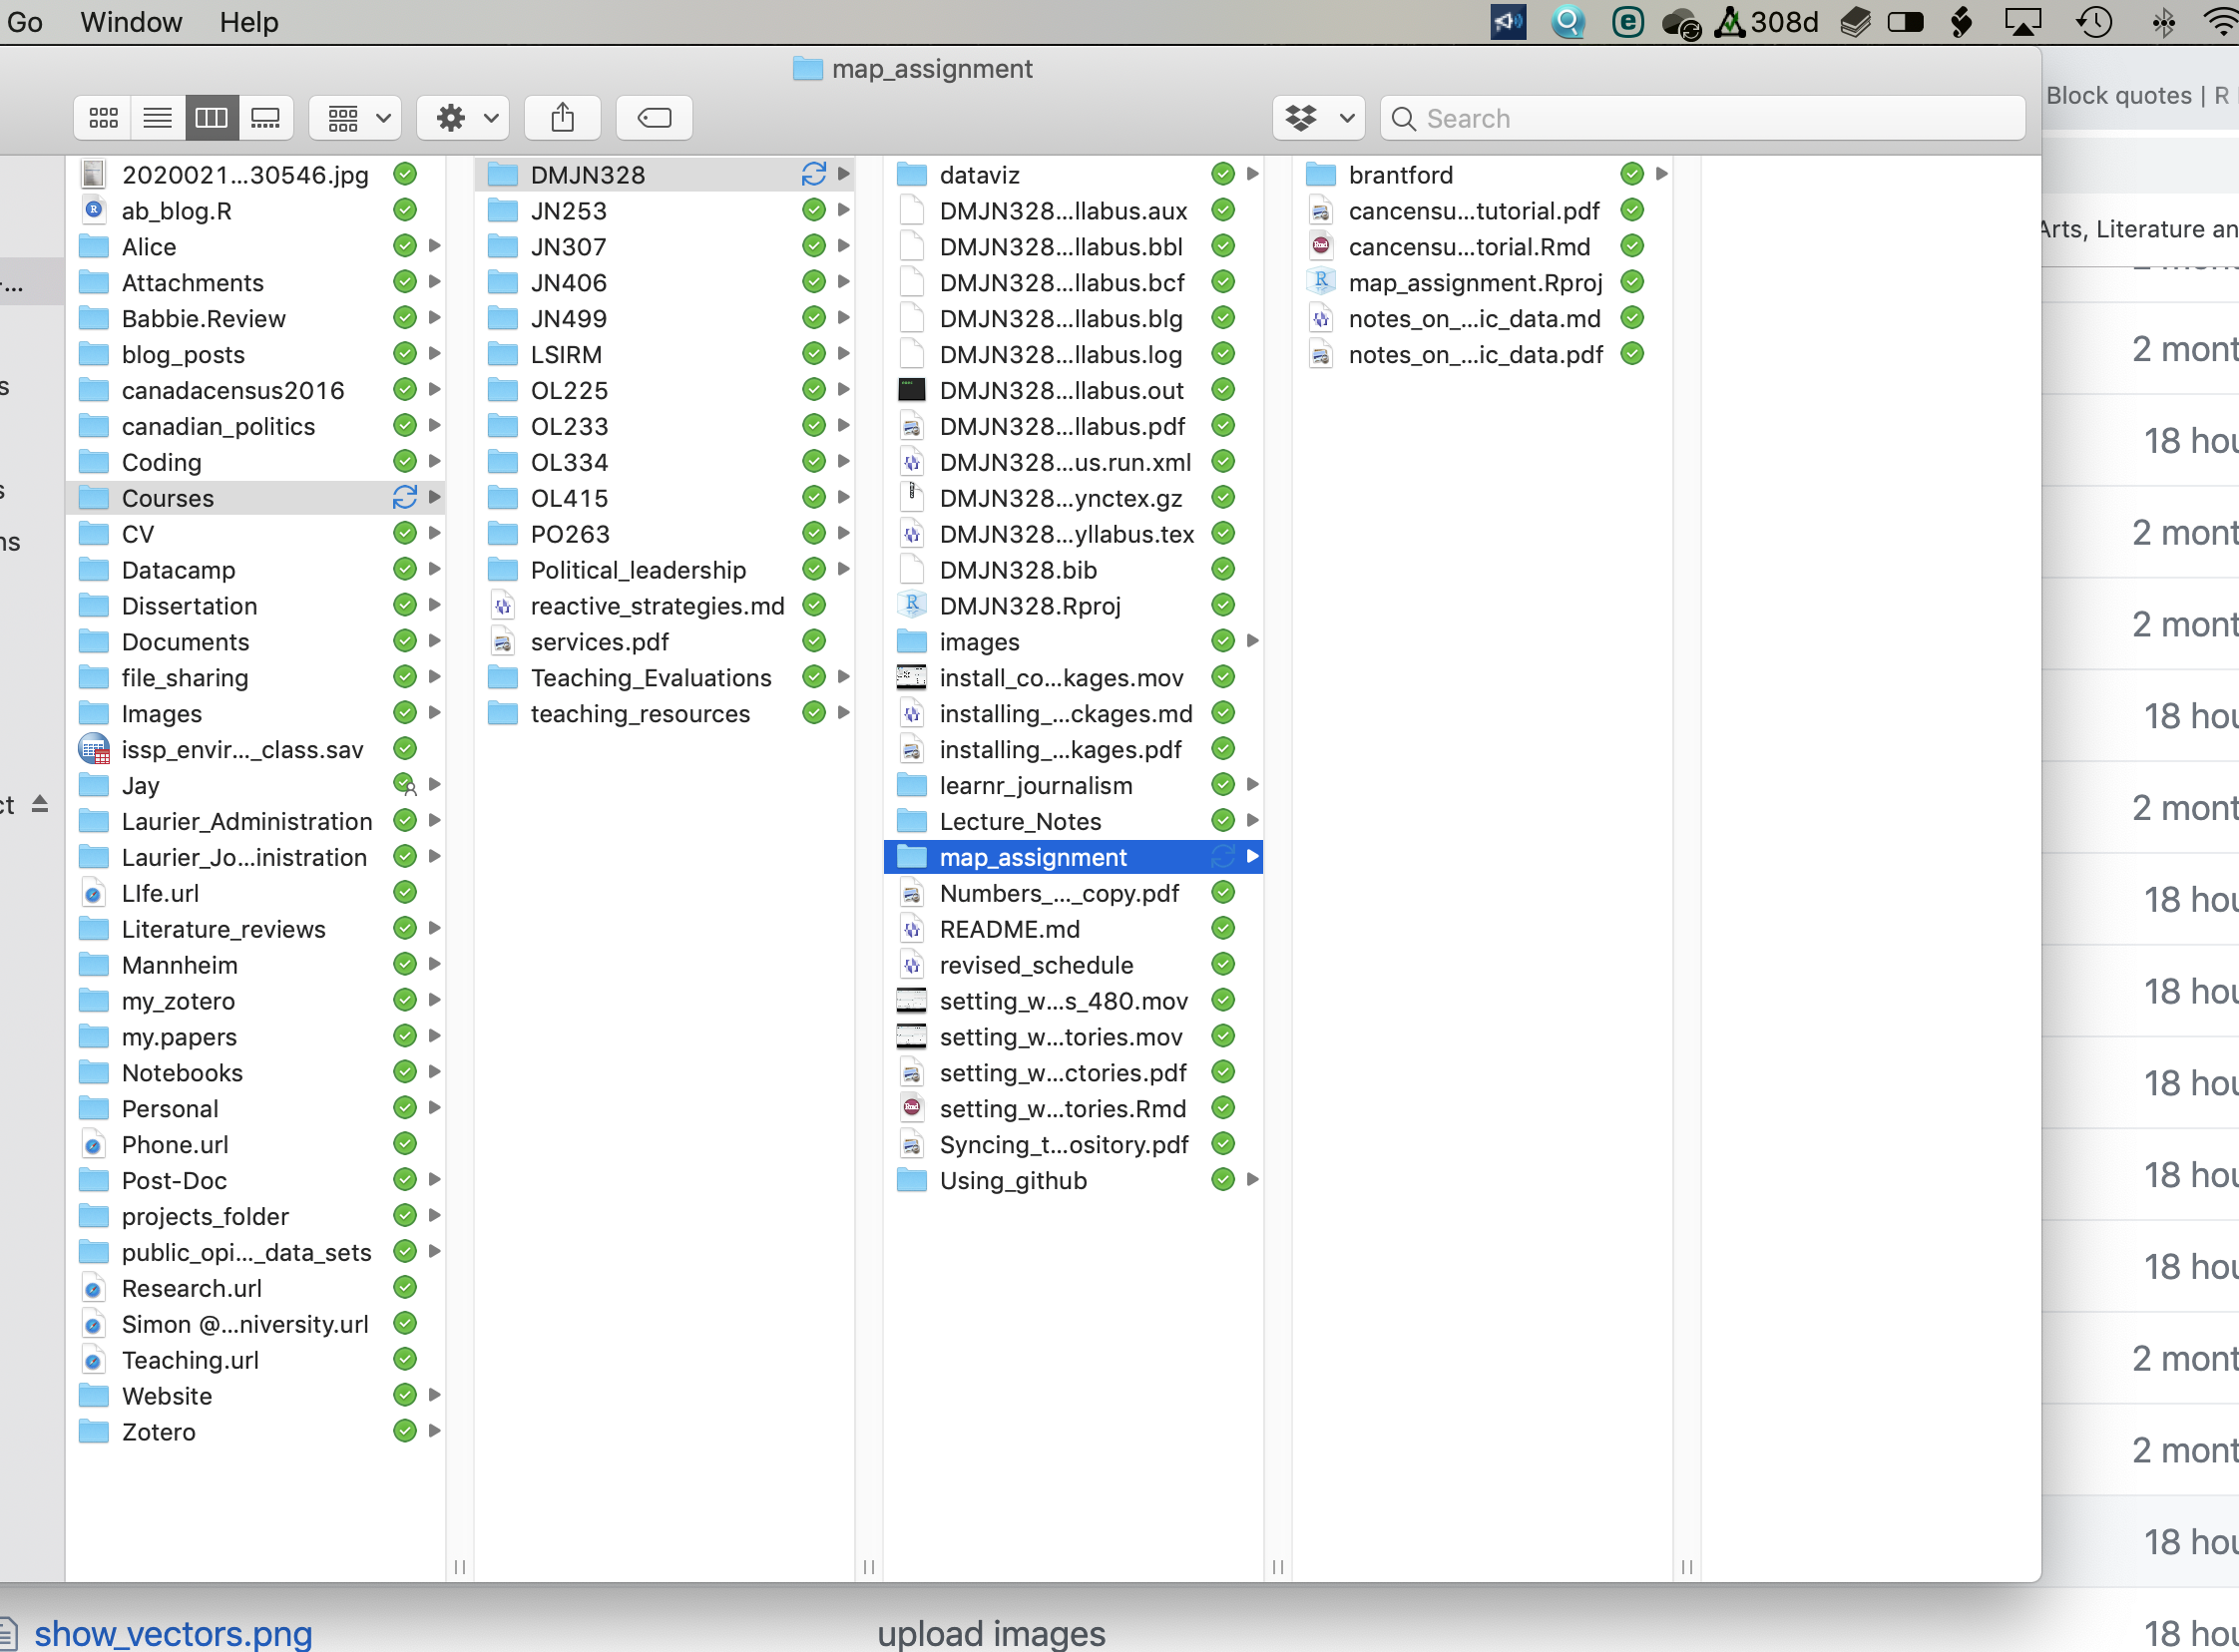
\includegraphics[width=0.5\linewidth]{images/map_assignment} \end{center}

Open the .Rproj file with RStudio.

If not, make your own folder in the course folder, call it whatever you
want and make an RStudio Project file in that folder.

\hypertarget{using-census-mapper}{%
\section{Using Census Mapper}\label{using-census-mapper}}

\href{http://www.censusmapper.ca}{Census Mapper} is an open source
project that makes it easier to access Statistics Canada's vast troves
of census data and link it to geographical files for Canada to make it
easier to visualize Canadian census data. It is meant to work seamlessly
with R.

\hypertarget{installing-the-package-and-loading-the-library}{%
\subsection{Installing the package and loading the
library}\label{installing-the-package-and-loading-the-library}}

As with everything, we need to install packages and load them.

Open an R Script (or you can open the pre-made cancensus\_tutorial.R
script that is in the \texttt{map\ assignment} folder)

You can start with these commands to install census mapper and load the
library.

Note, any code snippets that appear in this document are formatted so
that you should be able to copy and paste them into an R script.

\begin{Shaded}
\begin{Highlighting}[]
\KeywordTok{install.packages}\NormalTok{(}\StringTok{"censusmapper"}\NormalTok{)}
\KeywordTok{library}\NormalTok{(censusmapper)}
\end{Highlighting}
\end{Shaded}

\hypertarget{getting-an-api}{%
\subsection{Getting an API}\label{getting-an-api}}

While it is free and open source, it is necessary to register for an
API. Click on the top-right of the website to login and get an API.

\begin{Shaded}
\begin{Highlighting}[]
\KeywordTok{include\_graphics}\NormalTok{(}\StringTok{"images/get\_api.png"}\NormalTok{)}
\end{Highlighting}
\end{Shaded}

\begin{center}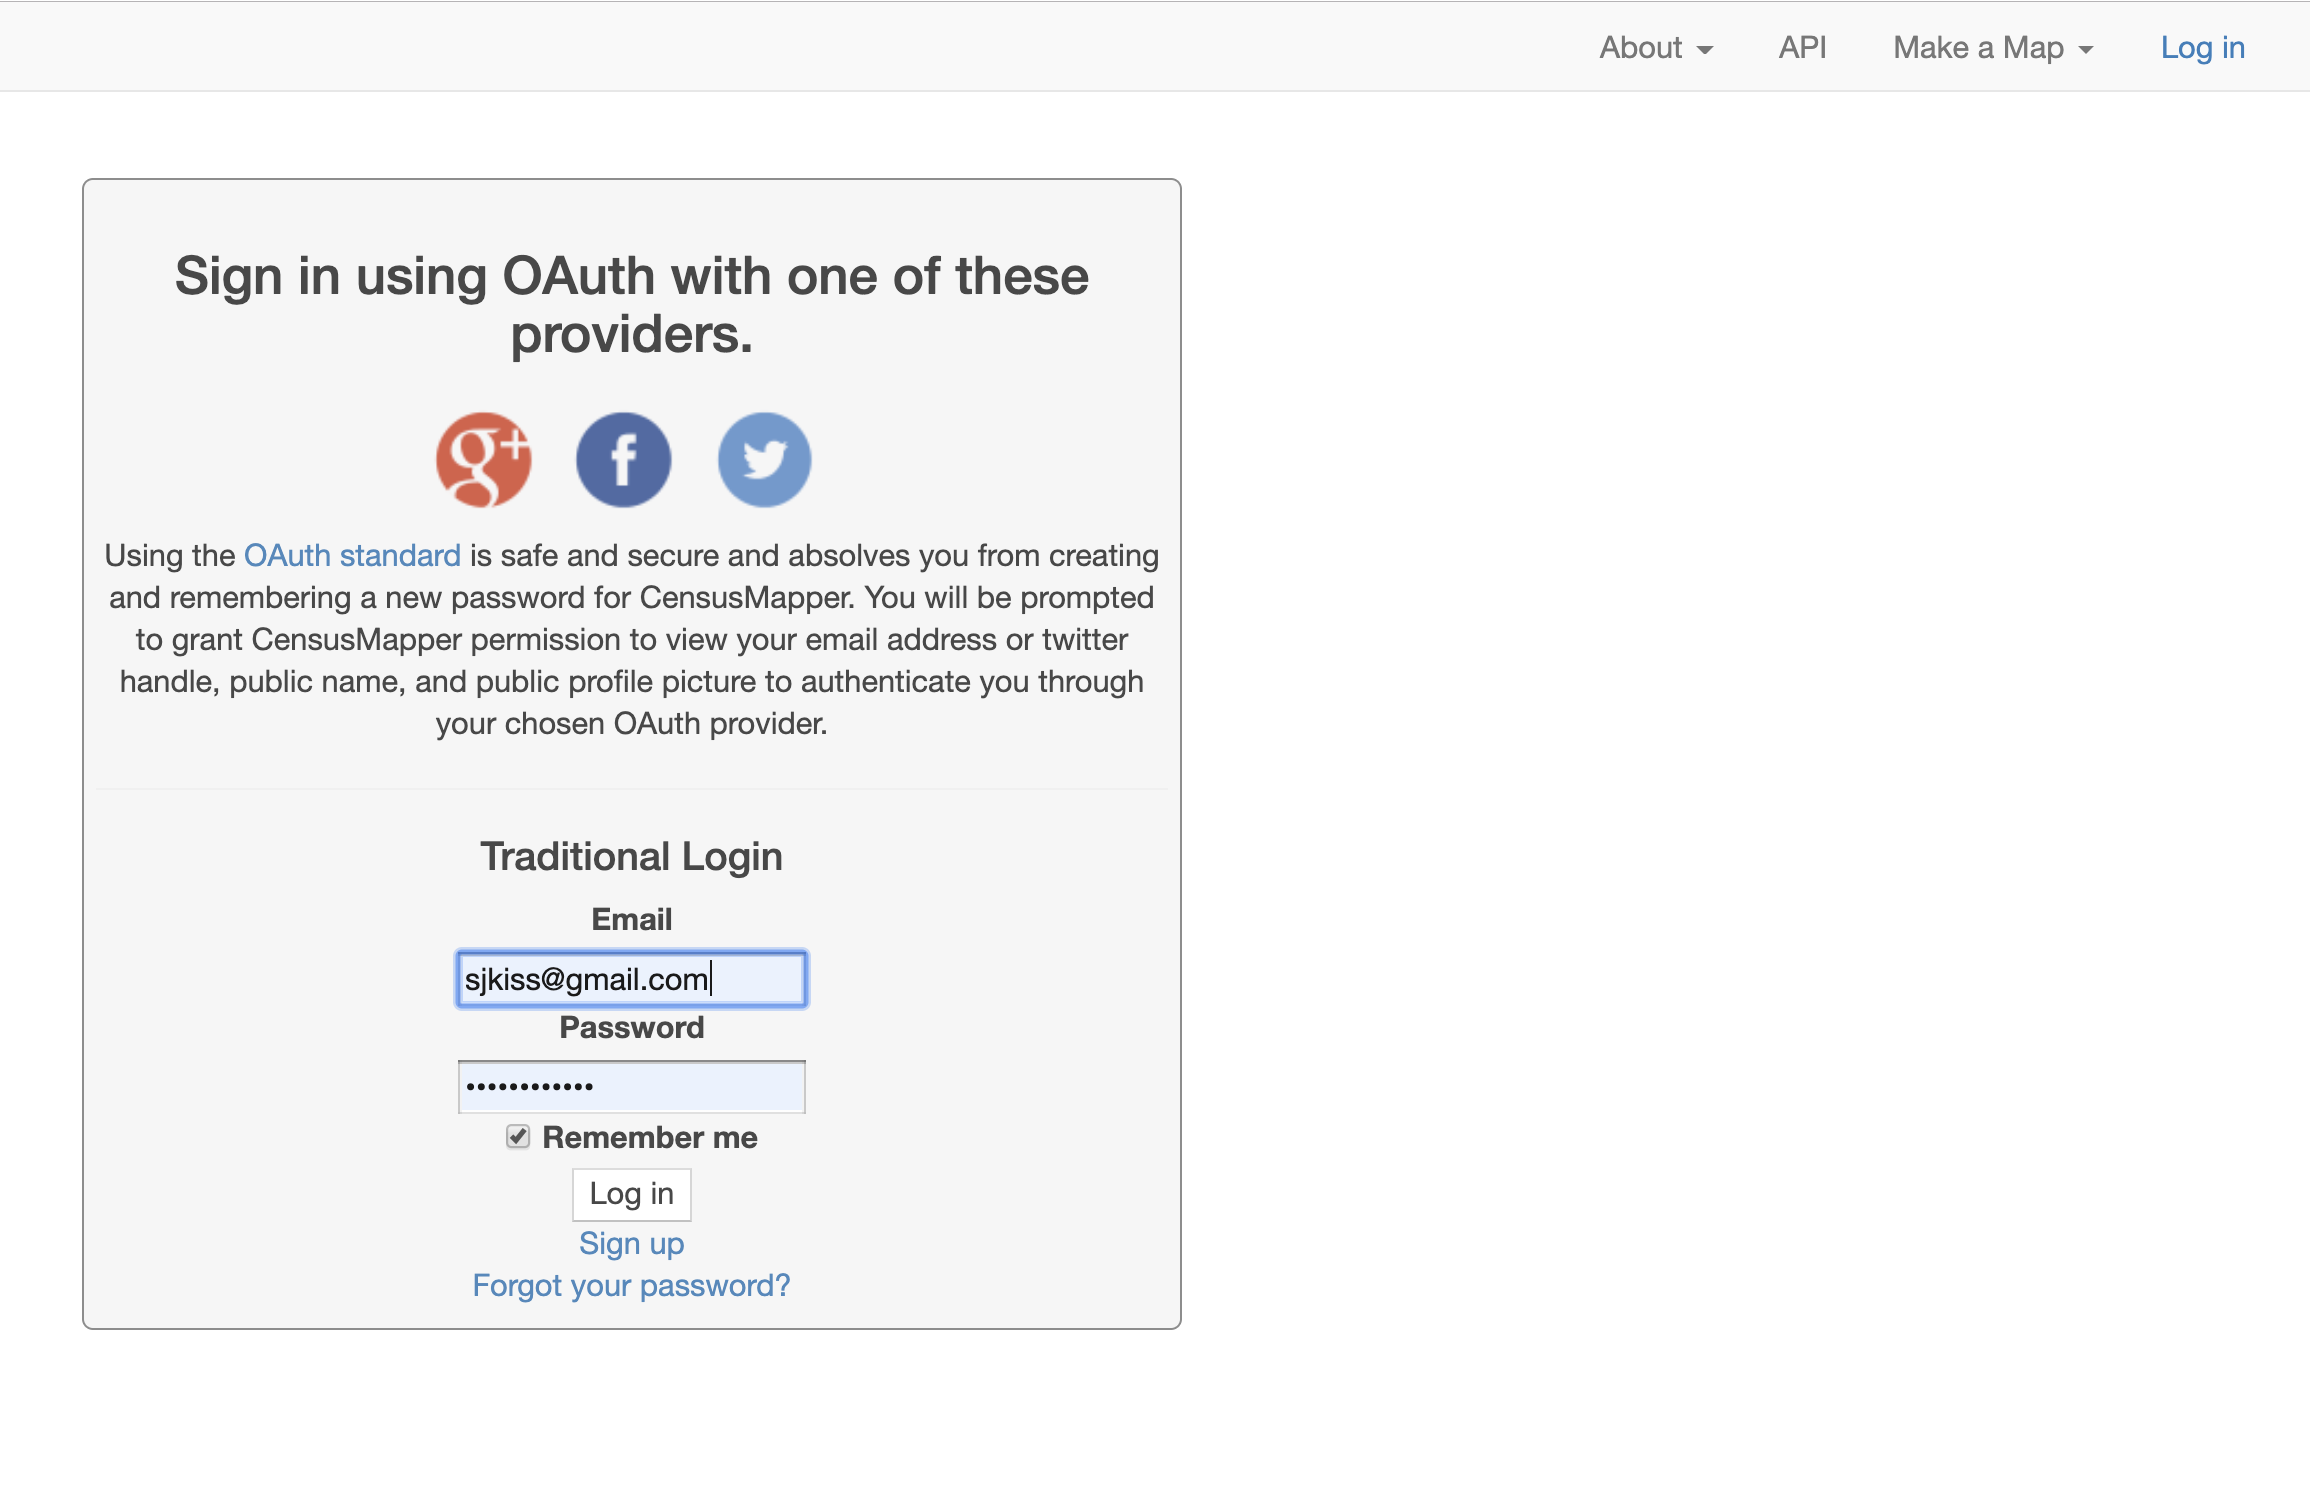
\includegraphics[width=0.5\linewidth]{images/get_api} \end{center}

The API should look something like this.

\begin{Shaded}
\begin{Highlighting}[]
\KeywordTok{include\_graphics}\NormalTok{(}\StringTok{"https://raw.githubusercontent.com/sjkiss/DMJN328/master/images/api.png"}\NormalTok{)}
\end{Highlighting}
\end{Shaded}

\begin{center}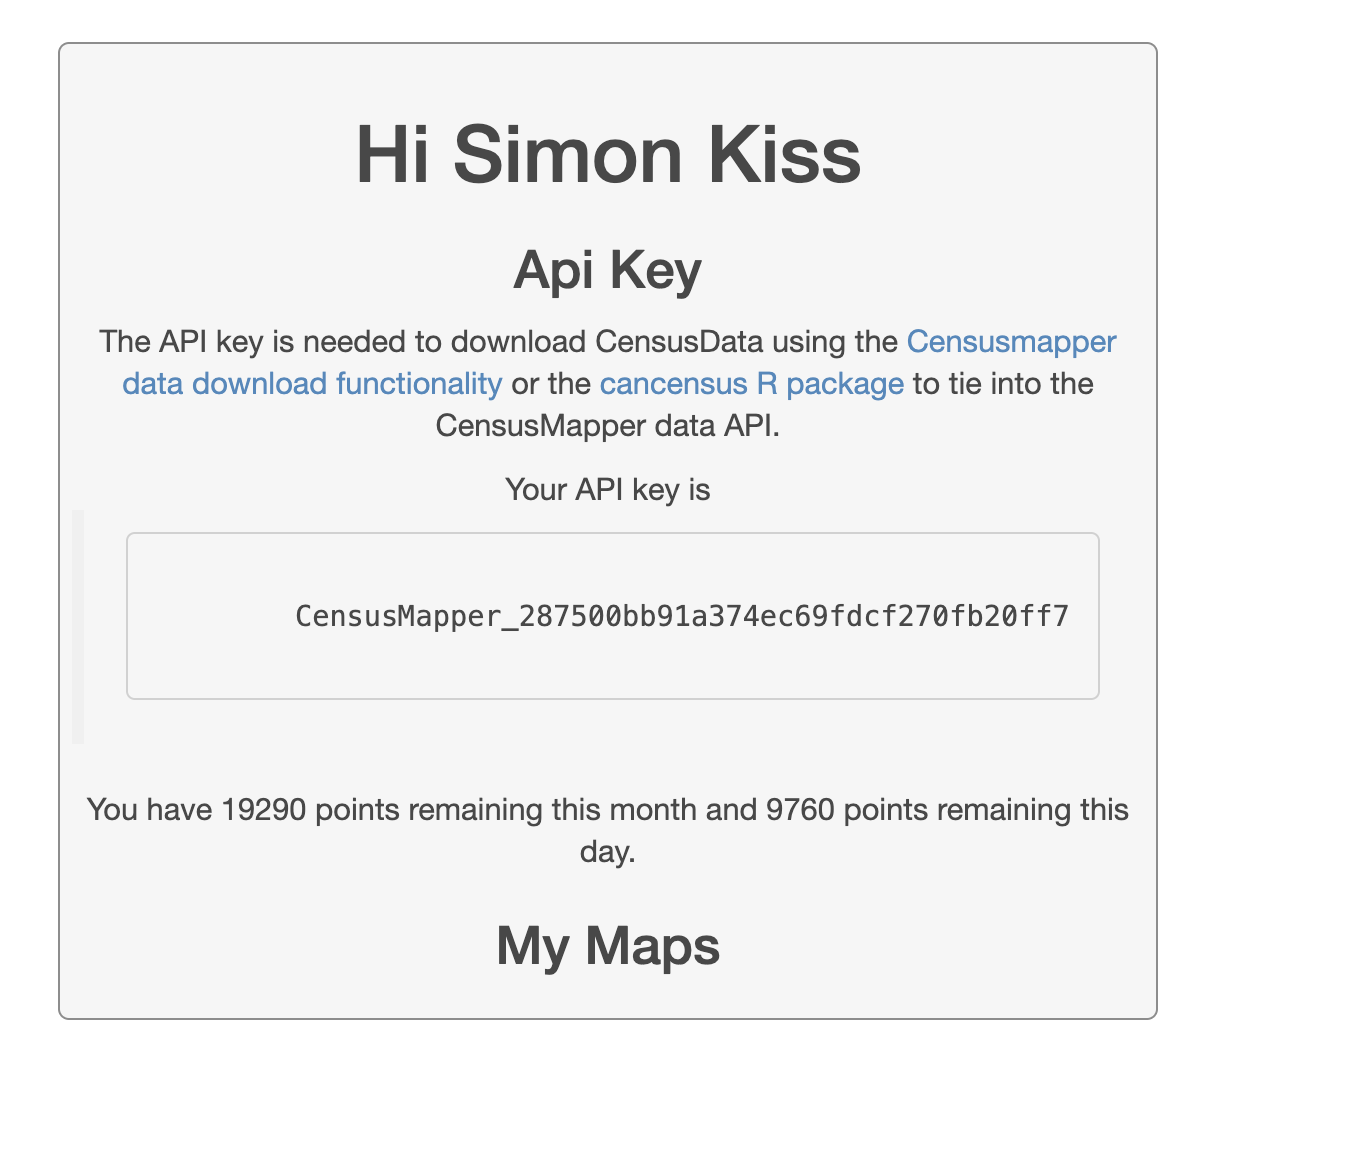
\includegraphics[width=0.5\linewidth]{https://raw.githubusercontent.com/sjkiss/DMJN328/master/images/api} \end{center}

\hypertarget{using-your-api-in-r}{%
\subsection{Using your API in R}\label{using-your-api-in-r}}

There are two ways to use your API: temporary and permanent.

\hypertarget{temporary}{%
\subsubsection{Temporary}\label{temporary}}

The temporary way is to insert the following command at the top of any
script you write that interacts with census mapper. \textbf{Of course,
you need to insert your own API key after the \texttt{=} sign.} The one
below is a modified version of my own, so it won't work.

\begin{Shaded}
\begin{Highlighting}[]
\KeywordTok{options}\NormalTok{(}\DataTypeTok{cancensus.api\_key =} \StringTok{"CensusMapper\_287500bb91a374ec69fdcf27"}\NormalTok{)}
\end{Highlighting}
\end{Shaded}

After that, any commands you run in that script will interact with
Census Mapper nicely.

The downside to the temporary approach is: 1) you need to do it every
time you write a script to get data or files from Census Mapper and 2)
if you share your code with anyone then you will expose your API. It's
not a big deal, but it's something.

\hypertarget{permanent}{%
\subsubsection{Permanent}\label{permanent}}

The permanent approach sets your cancensus API inside R permanently, or
as long as you have this computer. The way you do it is to open an
invisible file called \texttt{.Rprofile} on your computer and insert the
options command in there.

The following command opens \texttt{.Rprofile} (or makes it if it does
not already exist).

\begin{Shaded}
\begin{Highlighting}[]
\KeywordTok{file.edit}\NormalTok{(}\KeywordTok{file.path}\NormalTok{(}\StringTok{"\textasciitilde{}/.Rprofile"}\NormalTok{))}
\end{Highlighting}
\end{Shaded}

This is what mine looks like. Lines 1:3 are just notes for myself, line
4 is a little command that I use frequently and lines 5 and 6 are my
cancensus options.

\begin{Shaded}
\begin{Highlighting}[]
\KeywordTok{include\_graphics}\NormalTok{(}\StringTok{"images/rprofile.png"}\NormalTok{)}
\end{Highlighting}
\end{Shaded}

\begin{center}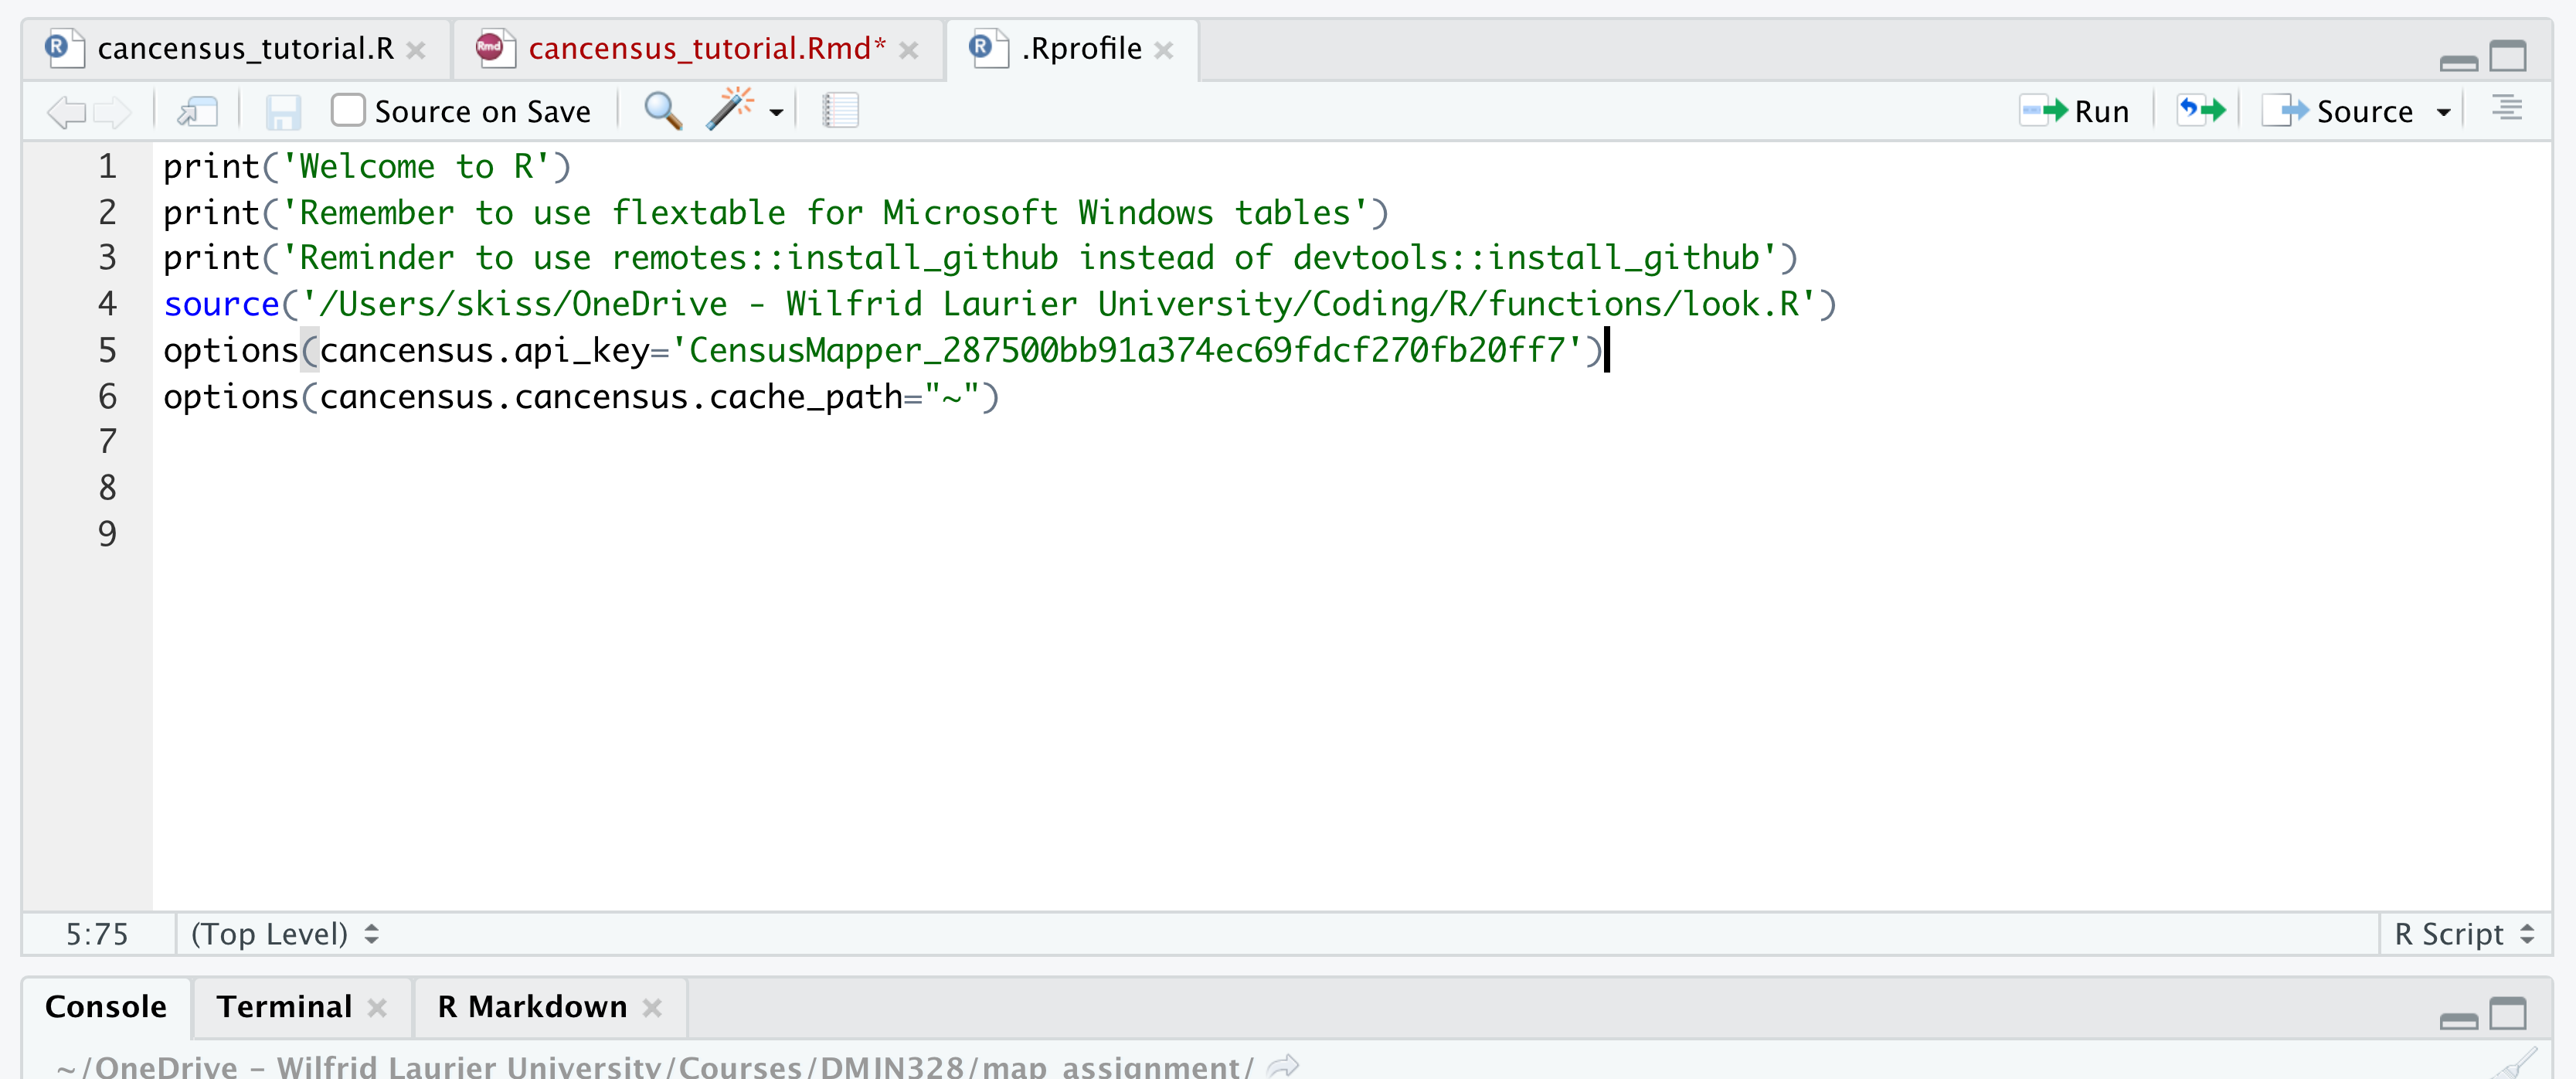
\includegraphics[width=0.5\linewidth]{images/rprofile} \end{center}

So, in your \texttt{.Rprofile} file, just plunk the \texttt{options()}
command with your api key, just like this and save it the file.

\begin{Shaded}
\begin{Highlighting}[]
\KeywordTok{options}\NormalTok{(}\DataTypeTok{cancensus.api\_key =} \StringTok{"CensusMapper\_287500bb91a374ec69fdcf270fb2"}\NormalTok{)}
\end{Highlighting}
\end{Shaded}

\hypertarget{censusmapper-cache}{%
\subsubsection{CensusMapper Cache}\label{censusmapper-cache}}

As you can imagine, downloading geographic files and Statistis Canada
data can involve quite a lot of data. This can: a) take a long time and
b) overload CensusMapper and Statistics Canada. To minimize the burden
on everyone, it is recommended (but not necessary) to also set a
\emph{cache} for census mapper data.

A cache is just like a food cache; a place to store something you might
need in the future.

So, in this case, you set a cancensus cache as directory on your
computer. When you download data from cancensus once, then it will be
stored there; if you need to run your script again, the cancensus
package will \emph{first} look in the cache to see if it is there,
allowing you to not go through the hassle of downloading the information
from the internet again.

This step is \emph{optional} but, for obvious reasons, recommended and
will probably make your life easier.

You set the cache directory the exact same way as setting the API.

Note that you get to choose where you want to put your cache. I find it
pretty unobtrusive just to put it in your root user directory, but it's
up to you.

To set it \emph{temporarily}, enter this command at the top of your
script. Note the \texttt{\textasciitilde{}} is Mac-speak for the user's
home directory. This \emph{should} work on a PC, but it might not. You
\emph{might} need to play with this a little bit, if you have a PC.

\begin{Shaded}
\begin{Highlighting}[]
\KeywordTok{options}\NormalTok{(}\DataTypeTok{cancensus.cancensus.cache\_path =} \StringTok{"\textasciitilde{}"}\NormalTok{)}
\end{Highlighting}
\end{Shaded}

To set it \emph{permanently}, enter the same command in your
\texttt{.rprofile} folder, following the steps above, save and restart.

\emph{If you have gone the permanent route and modified your .Rprofile
file, you need to restart RStudio for the changes to take effect}

\hypertarget{getting-the-data-out-of-census-mapper.}{%
\subsection{Getting the data out of Census
Mapper.}\label{getting-the-data-out-of-census-mapper.}}

Now we can go over to \href{http://censusmapper.ca}{} to get our
geography and data files.

Remember that to make our map, we need both some geography files and
some data to visualize.

\hypertarget{geography}{%
\subsubsection{Geography}\label{geography}}

To select the geographic area you want to work with, play with the
cursor to zoom to a region you are interested in.

If you click on ``Region Selection'' you can zoom quickly to different
levels of geography, e.g.~Province, census division, census
sub-division, census metropolitan area, whatever. I find this
convenient.

When you have a geographic boundary area that you are interested in
playing with, select it and it should turn \emph{blue}. If you click the
same area again, it should deselct the region. this is what it looks
like if you have selected Ontario.

\begin{Shaded}
\begin{Highlighting}[]
\KeywordTok{include\_graphics}\NormalTok{(}\StringTok{"images/selecting\_ontario.png"}\NormalTok{)}
\end{Highlighting}
\end{Shaded}

\begin{center}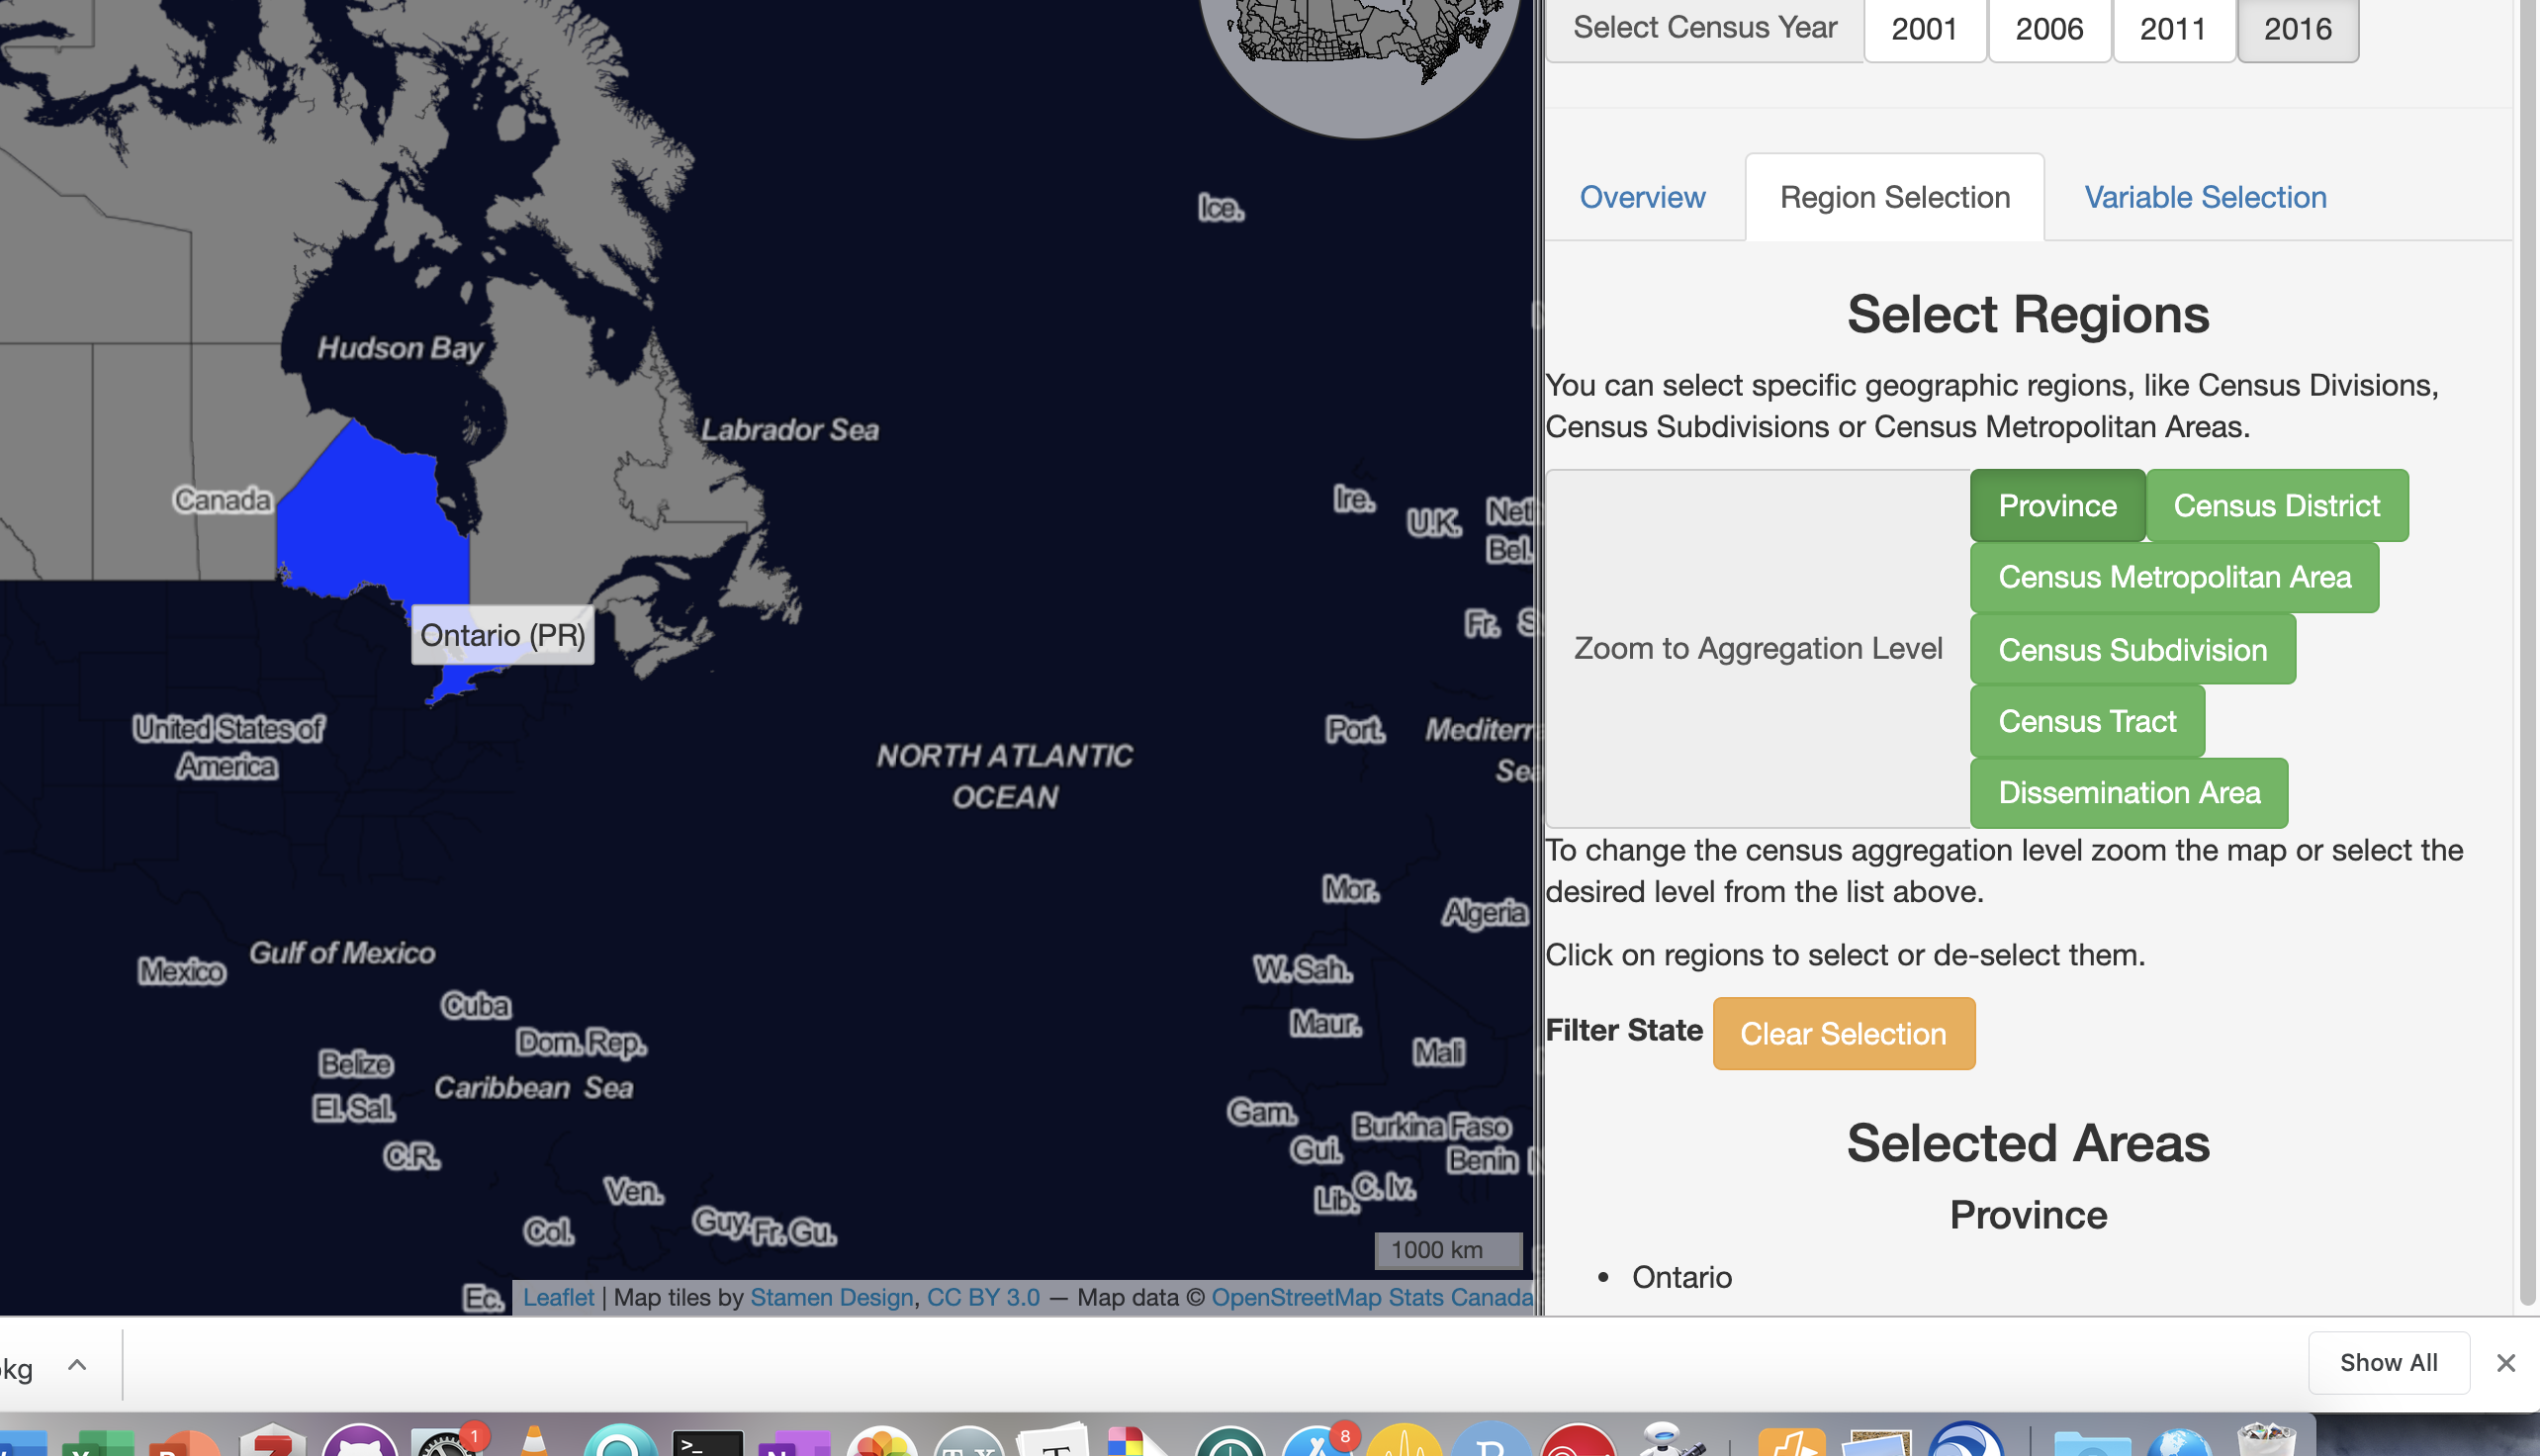
\includegraphics[width=0.5\linewidth]{images/selecting_ontario} \end{center}

Please note: when you select a geographic region, you will still be able
to get the boundary files and data from \emph{sub-units}. So, in the
image, I have selected Ontario, but at the next step, I will be able to
get data and boundaries on sub-units (e.g.~census sub-divisions for all
of Ontario, or even all the census tracts). Here, I have just excluded
other provinces.

So this is a choice you get to make. One thing to keep in mind, the
larger the geographic unit that you select, the more data you will be
downloading.

I am going to select Kitchener, so I'm going to zoom in on the Census
Metropolitan Area level, drag the map to about the KW area and select
Kitchener.

\begin{Shaded}
\begin{Highlighting}[]
\KeywordTok{include\_graphics}\NormalTok{(}\StringTok{"images/select\_kitchener.png"}\NormalTok{)}
\end{Highlighting}
\end{Shaded}

\begin{center}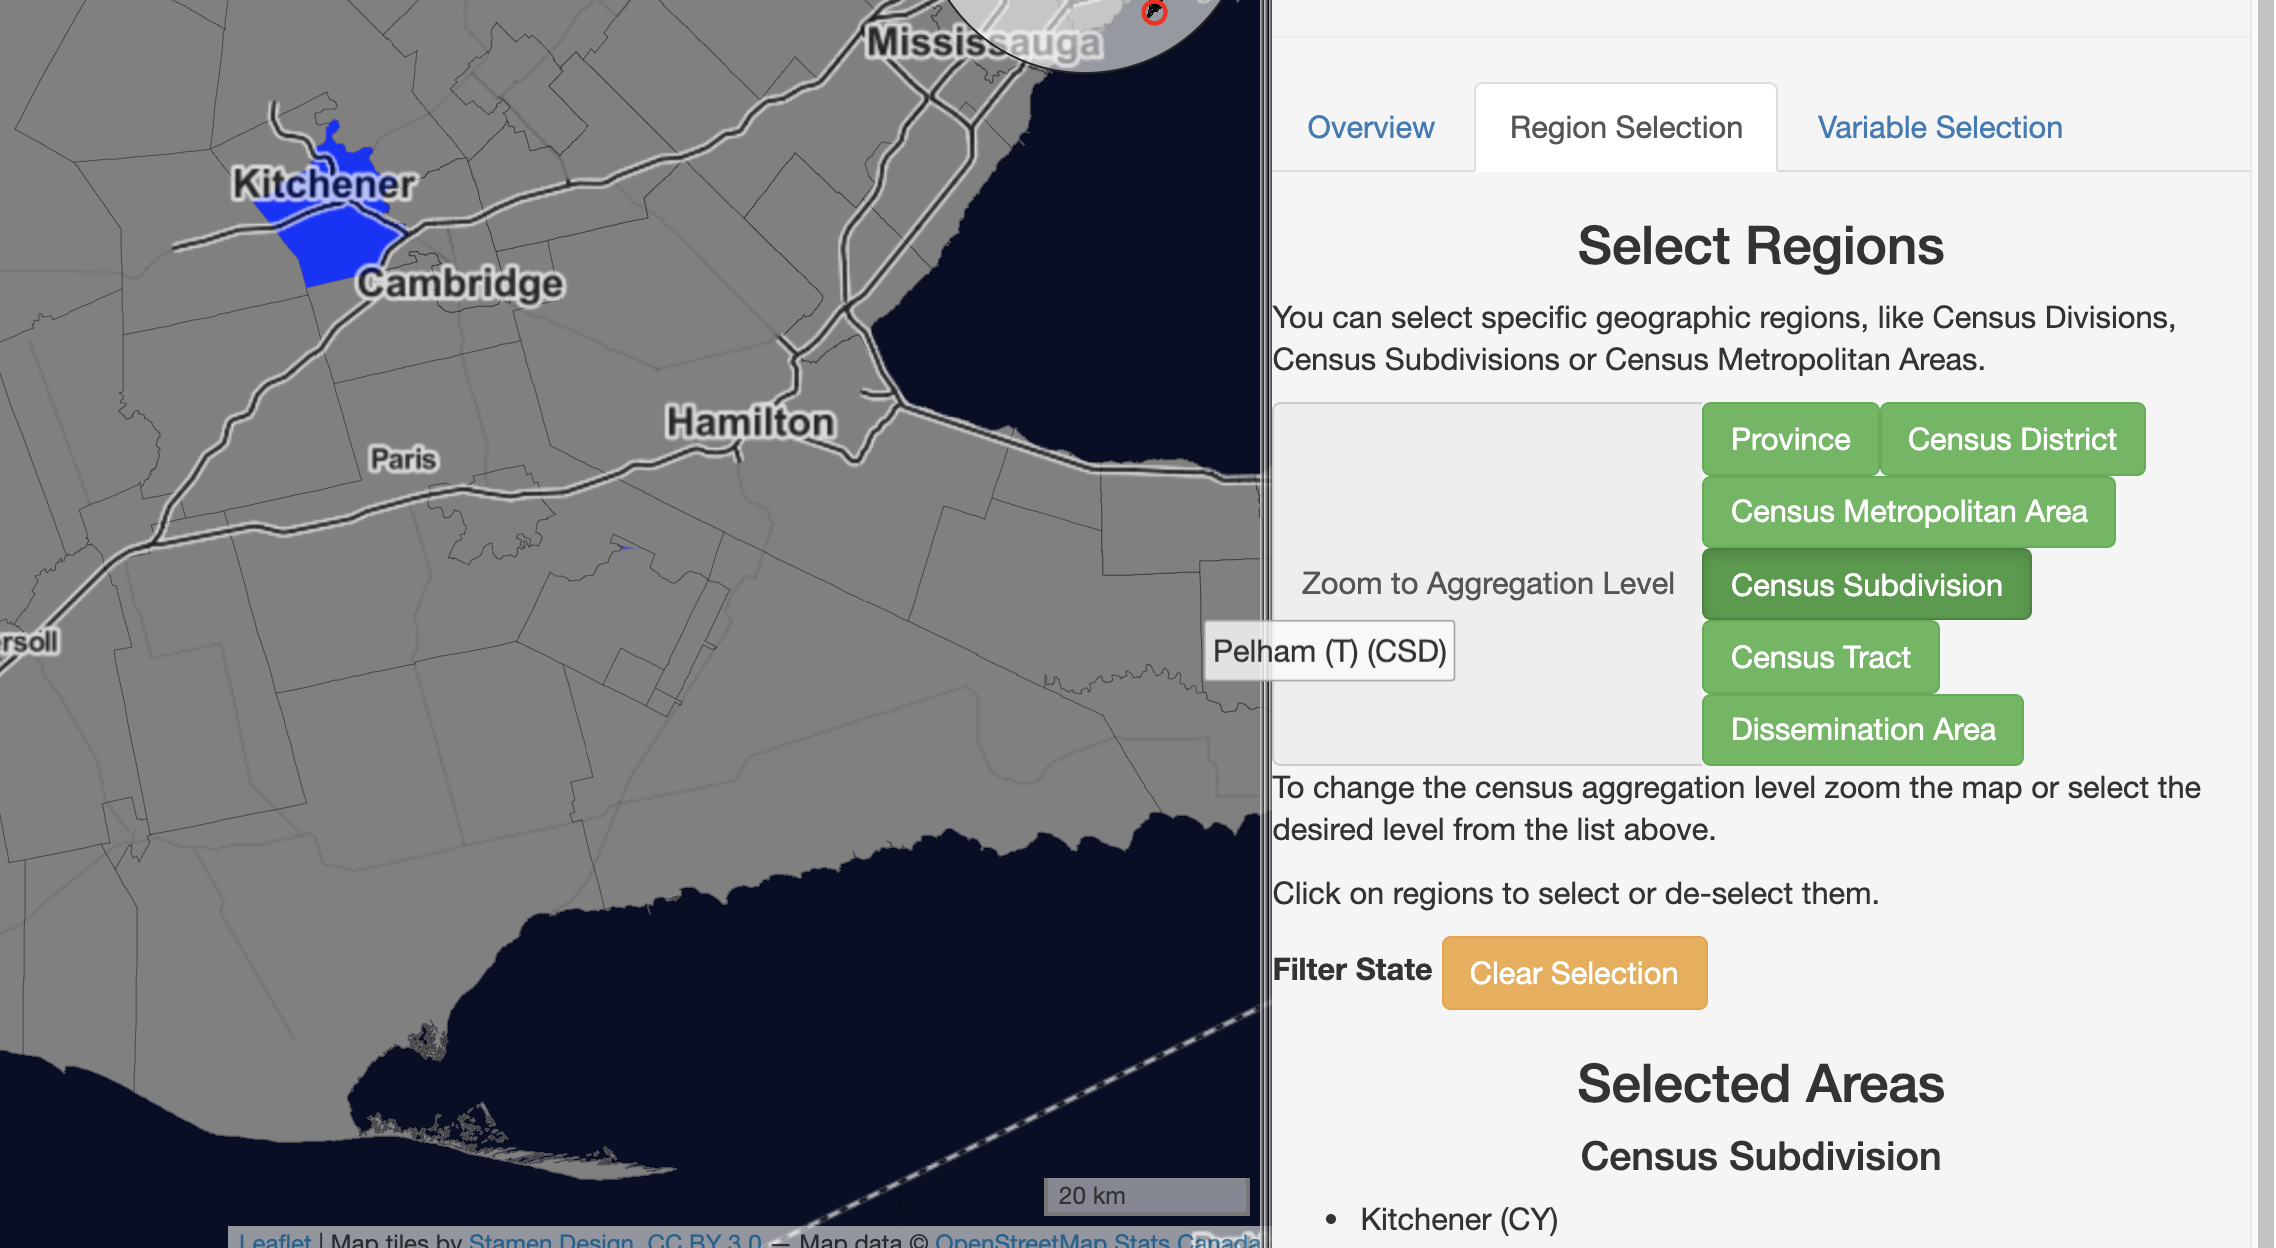
\includegraphics[width=0.5\linewidth]{images/select_kitchener} \end{center}

Note that I had to select ``Clear Selection'' first to deselect Ontario,
and then select ``Kitchener''.

If I jump over to ``Overview'' I'm going to get a screen that looks
below. There's some useful information here.

\begin{Shaded}
\begin{Highlighting}[]
\KeywordTok{include\_graphics}\NormalTok{(}\StringTok{"images/select\_region.png"}\NormalTok{)}
\end{Highlighting}
\end{Shaded}

\begin{center}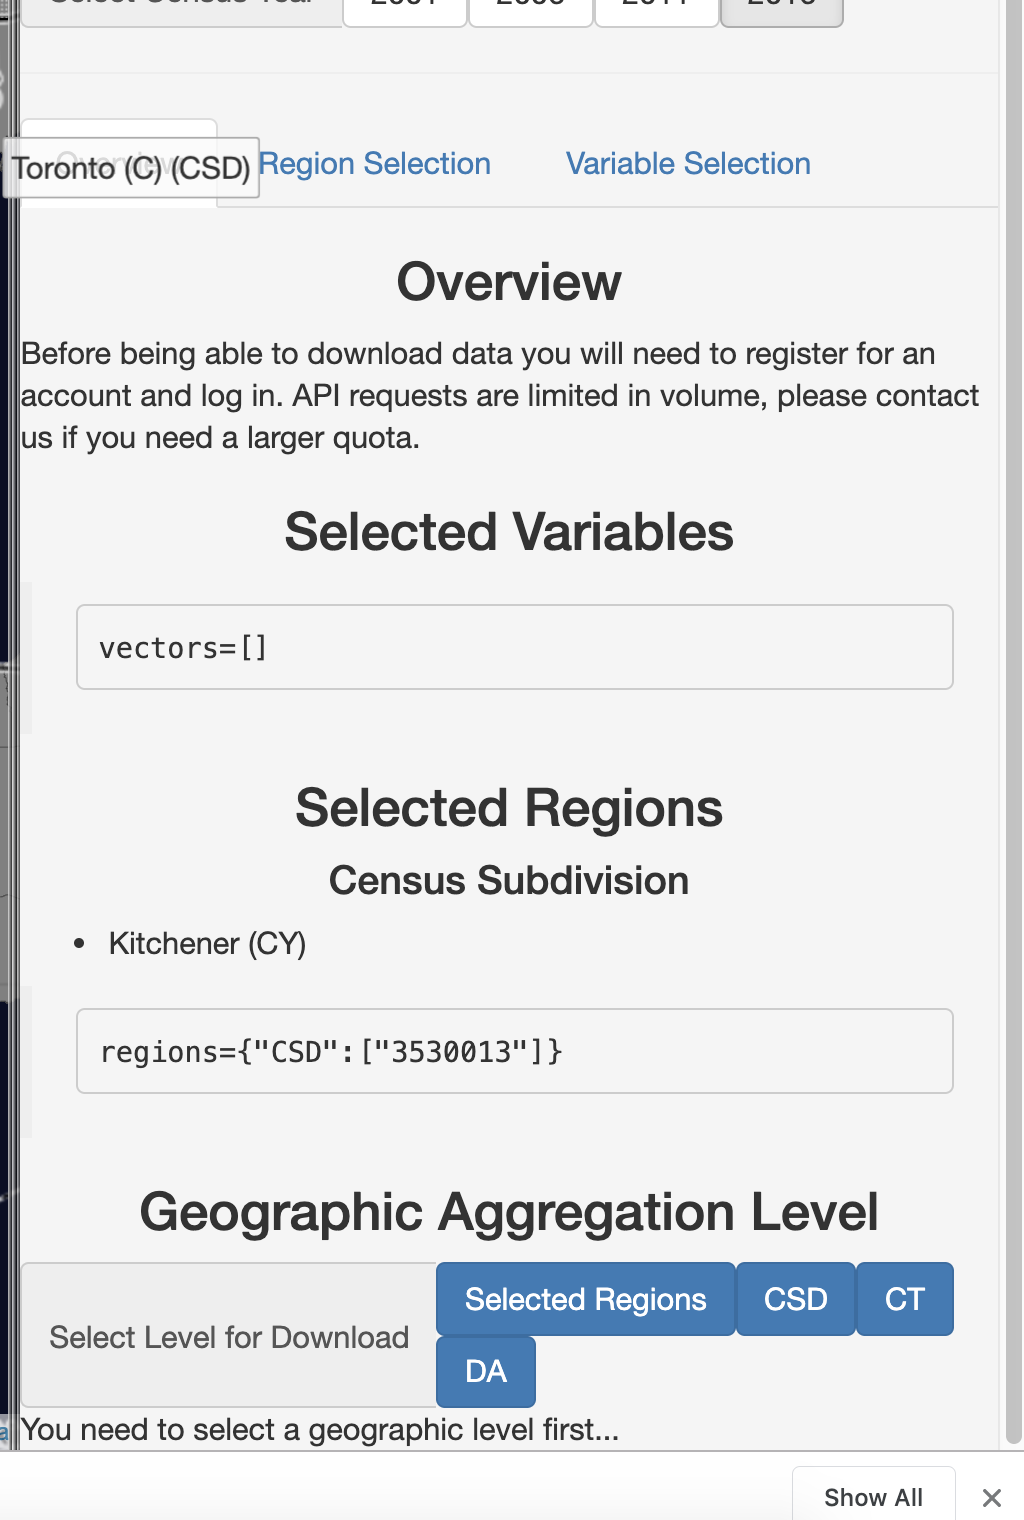
\includegraphics[width=0.5\linewidth]{images/select_region} \end{center}

Notice under ``Selected Variables'' it says \texttt{vectors={[}{]}}.
That is because we have not yet selected any data to download.

And under ``Selected Regions'', it says that we have selected Kitchener
(CY) and that \texttt{regions=\{"CSD":{[}"3530013"{]}\}.\ The}regions`
stuff is code for Census Subdivision (CSD) 3530013.

The more you play with STatistics Canada's data, the more you will learn
how it works, but basically, the CSD code is made of a province code
(Ontario = 35), a two-digit Census Division code (Waterloo Region = 30)
and a 3-digit Census Sub-division code (City of Kitchener = 013).

So, Statistics Canada has a very systematic way of coding Canada's
geography. Kitchener is always through all of StatsCan's data coded as
35300013.

Under Geographic Aggregation Level, there isn't really anything
selected. Here, we can select what level of data we want to visualize
and what boundaries we want to draw. Because we have only selected the
City of Kitchener (which is a Census Sub-Division) there are only three
options that we can download:

\begin{enumerate}
\def\labelenumi{\arabic{enumi}.}
\tightlist
\item
  CSD (Census Subdivision) which will download the outer boundaries of
  the CSD Kitchener
\item
  CT (Census Tracts) which are about maybe ward-level boundaries inside
  the City of Ktichener
\item
  DA (Dissemination Areas) which are almost block-level boundaries
  inside Kitchener.
\end{enumerate}

Obviously option 3 will give us the most fine-grained view of the City
of Kitchener, but you might not get as much data.

I raised this in class the ohter day, but in looking at it, I see that
there actually is quite a lot of data. So, let's do it.

Let's select DA.

\begin{Shaded}
\begin{Highlighting}[]
\KeywordTok{include\_graphics}\NormalTok{(}\StringTok{"images/selecting\_dissemination\_areas.png"}\NormalTok{)}
\end{Highlighting}
\end{Shaded}

\begin{center}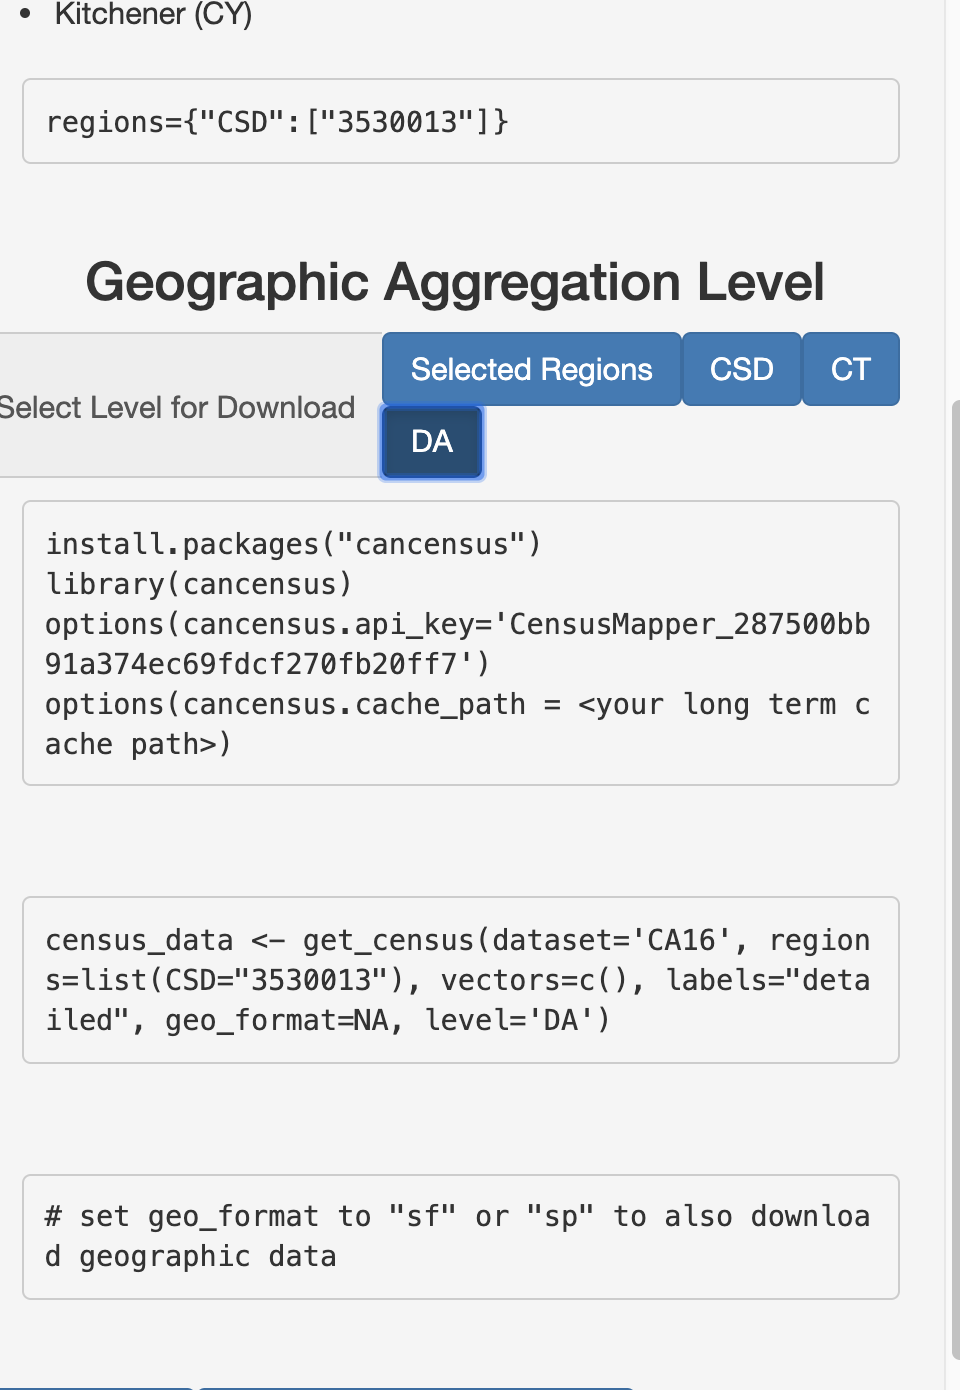
\includegraphics[width=0.5\linewidth]{images/selecting_dissemination_areas} \end{center}

Then go back to overview. If you look at the bottom, there is some R
code there and it should look just like this.

\begin{Shaded}
\begin{Highlighting}[]
\NormalTok{census\_data <{-}}\StringTok{ }\KeywordTok{get\_census}\NormalTok{(}\DataTypeTok{dataset =} \StringTok{"CA16"}\NormalTok{, }\DataTypeTok{regions =} \KeywordTok{list}\NormalTok{(}\DataTypeTok{CSD =} \StringTok{"3530013"}\NormalTok{), }\DataTypeTok{vectors =} \KeywordTok{c}\NormalTok{(), }
    \DataTypeTok{labels =} \StringTok{"detailed"}\NormalTok{, }\DataTypeTok{geo\_format =} \OtherTok{NA}\NormalTok{, }\DataTypeTok{level =} \StringTok{"DA"}\NormalTok{)}
\end{Highlighting}
\end{Shaded}

I am going to modify it slightly and comment it so we know what is going
on.

\begin{Shaded}
\begin{Highlighting}[]
\CommentTok{\# Instead of saving it as census\_data, I am saving it as kitchener, for ease of}
\CommentTok{\# memory. dataset=CA16 says get data or boundary files from the 2016 Census}
\NormalTok{kitchener <{-}}\StringTok{ }\KeywordTok{get\_census}\NormalTok{(}\DataTypeTok{dataset =} \StringTok{"CA16"}\NormalTok{, }\DataTypeTok{regions =} \KeywordTok{list}\NormalTok{(}\DataTypeTok{CSD =} \StringTok{"3530013"}\NormalTok{), }\DataTypeTok{vectors =} \KeywordTok{c}\NormalTok{(), }
    \DataTypeTok{labels =} \StringTok{"detailed"}\NormalTok{, }\DataTypeTok{geo\_format =} \StringTok{"sf"}\NormalTok{, }\DataTypeTok{level =} \StringTok{"DA"}\NormalTok{)}
\end{Highlighting}
\end{Shaded}

This should leave us with an object called \texttt{kitchener} in our
environment.

Try this command.

\begin{Shaded}
\begin{Highlighting}[]
\KeywordTok{library}\NormalTok{(tidyverse)}
\KeywordTok{glimpse}\NormalTok{(kitchener)}
\end{Highlighting}
\end{Shaded}

\begin{verbatim}
## Observations: 314
## Variables: 11
## $ `Shape Area` <dbl> 0.78200, 0.33188, 0.56447, 0.18680, 0.16206, 0.15935, ...
## $ Type         <fct> DA, DA, DA, DA, DA, DA, DA, DA, DA, DA, DA, DA, DA, DA...
## $ Dwellings    <int> 230, 191, 254, 210, 199, 223, 306, 283, 185, 360, 226,...
## $ Households   <int> 223, 168, 244, 210, 194, 217, 284, 268, 185, 357, 215,...
## $ GeoUID       <chr> "35300097", "35300098", "35300099", "35300100", "35300...
## $ Population   <int> 588, 402, 552, 491, 425, 513, 584, 532, 459, 530, 374,...
## $ CD_UID       <chr> "3530", "3530", "3530", "3530", "3530", "3530", "3530"...
## $ CSD_UID      <chr> "3530013", "3530013", "3530013", "3530013", "3530013",...
## $ CT_UID       <chr> "5410024.00", "5410024.00", "5410023.00", "5410023.00"...
## $ CMA_UID      <chr> "35541", "35541", "35541", "35541", "35541", "35541", ...
## $ geometry     <MULTIPOLYGON [°]> MULTIPOLYGON (((-80.49342 4..., MULTIPOLY...
\end{verbatim}

So there you have it: the dissemination area boundary files for the city
of Kitchener. There are 314 observations (rows) of 11 variables. We can
go through them one-by-one beause it is quite informative.

\begin{enumerate}
\def\labelenumi{\arabic{enumi}.}
\tightlist
\item
  \texttt{Shape\ Area} - I \emph{think} this is the size of each
  dissemination area.
\item
  \texttt{Type} - is a factor (fct), and it just says that each row is a
  dissemination area (DA)
\item
  \texttt{Dwellings} - integer (int) variable that says how many
  dwellings are in each DA
\item
  \texttt{Households} - integer (int) variable that says how many
  households are in each. I don't quite understand the difference; one
  would have to read some documentation at Statistis Caanda.
\item
  GEOUID - character (so not a number) . From the looks of this, this
  looks like it is the unique identifier for each dissemination Area
  (more
  \href{https://www150.statcan.gc.ca/n1/pub/92f0138m/92f0138m2019001-eng.htm}{here})
\item
  Population - Integer (int) variable showing the population of each DA
\item
  CD\_UID - variable showing the census district identifier \texttt{35}
  for Ontario and \texttt{30} for the Census District of Region of
  Waterloo
\item
  CSD\_UID - variable showig the Census sub-division
  identifier:\texttt{35} for Ontario and \texttt{30} for the Census
  District of Region of Waterloo, and \texttt{013} for the CSD of
  Kitchener
\item
  CT\_UID - variable showing the Census Tract identifier for the CT that
  each DA is in. 10.CMA\_UID - variable showing the ID for the CMA
  (Census Metropolitan Area) that each DA is in.
  Kitchener-Waterloo-Cambridge is the CMA 35541 (\texttt{35} for Ontario
  and \texttt{541} ) for all of K-W-C.
\item
  geometry - there it; those are the geometry coordinates for each of
  the DAs.
\end{enumerate}

\hypertarget{drawing-the-map}{%
\subsection{Drawing the map}\label{drawing-the-map}}

Now it should be dead easy to draw the map, because it's \emph{exactly
the way it works in the lesson}.

\begin{Shaded}
\begin{Highlighting}[]
\KeywordTok{library}\NormalTok{(ggplot2)}
\KeywordTok{ggplot}\NormalTok{(kitchener, }\KeywordTok{aes}\NormalTok{(}\DataTypeTok{geometry =}\NormalTok{ geometry)) }\OperatorTok{+}\StringTok{ }\KeywordTok{geom\_sf}\NormalTok{()}
\end{Highlighting}
\end{Shaded}

\begin{center}\includegraphics[width=0.5\linewidth]{cancensus_tutorial_files/figure-latex/unnamed-chunk-3-1} \end{center}

When you download the boundary files for a region, it looks like you get
basic population data. So with just this command, we could fill in each
DA with the population \#s exactly the way that we did with the boston
data in the exercises.

\begin{Shaded}
\begin{Highlighting}[]
\KeywordTok{ggplot}\NormalTok{(kitchener, }\KeywordTok{aes}\NormalTok{(}\DataTypeTok{geometry =}\NormalTok{ geometry, }\DataTypeTok{fill =}\NormalTok{ Population)) }\OperatorTok{+}\StringTok{ }\KeywordTok{geom\_sf}\NormalTok{()}
\end{Highlighting}
\end{Shaded}

\begin{center}\includegraphics[width=0.5\linewidth]{cancensus_tutorial_files/figure-latex/unnamed-chunk-4-1} \end{center}

I'm going to stop there, because we've practiced different ways of
gussying up the map in the exercises, and it's pretty easy.

The next section talks about how to add different variables, other than
population via \texttt{cancensus}

\hypertarget{data}{%
\subsection{Data}\label{data}}

go back to the web browser and click on ``Variable Selection'' Honestly,
this product is so incredible it kind of makes your head spin. Bear with
me.

\begin{Shaded}
\begin{Highlighting}[]
\KeywordTok{include\_graphics}\NormalTok{(}\StringTok{"images/select\_kitchener\_variables.png"}\NormalTok{)}
\end{Highlighting}
\end{Shaded}

\begin{center}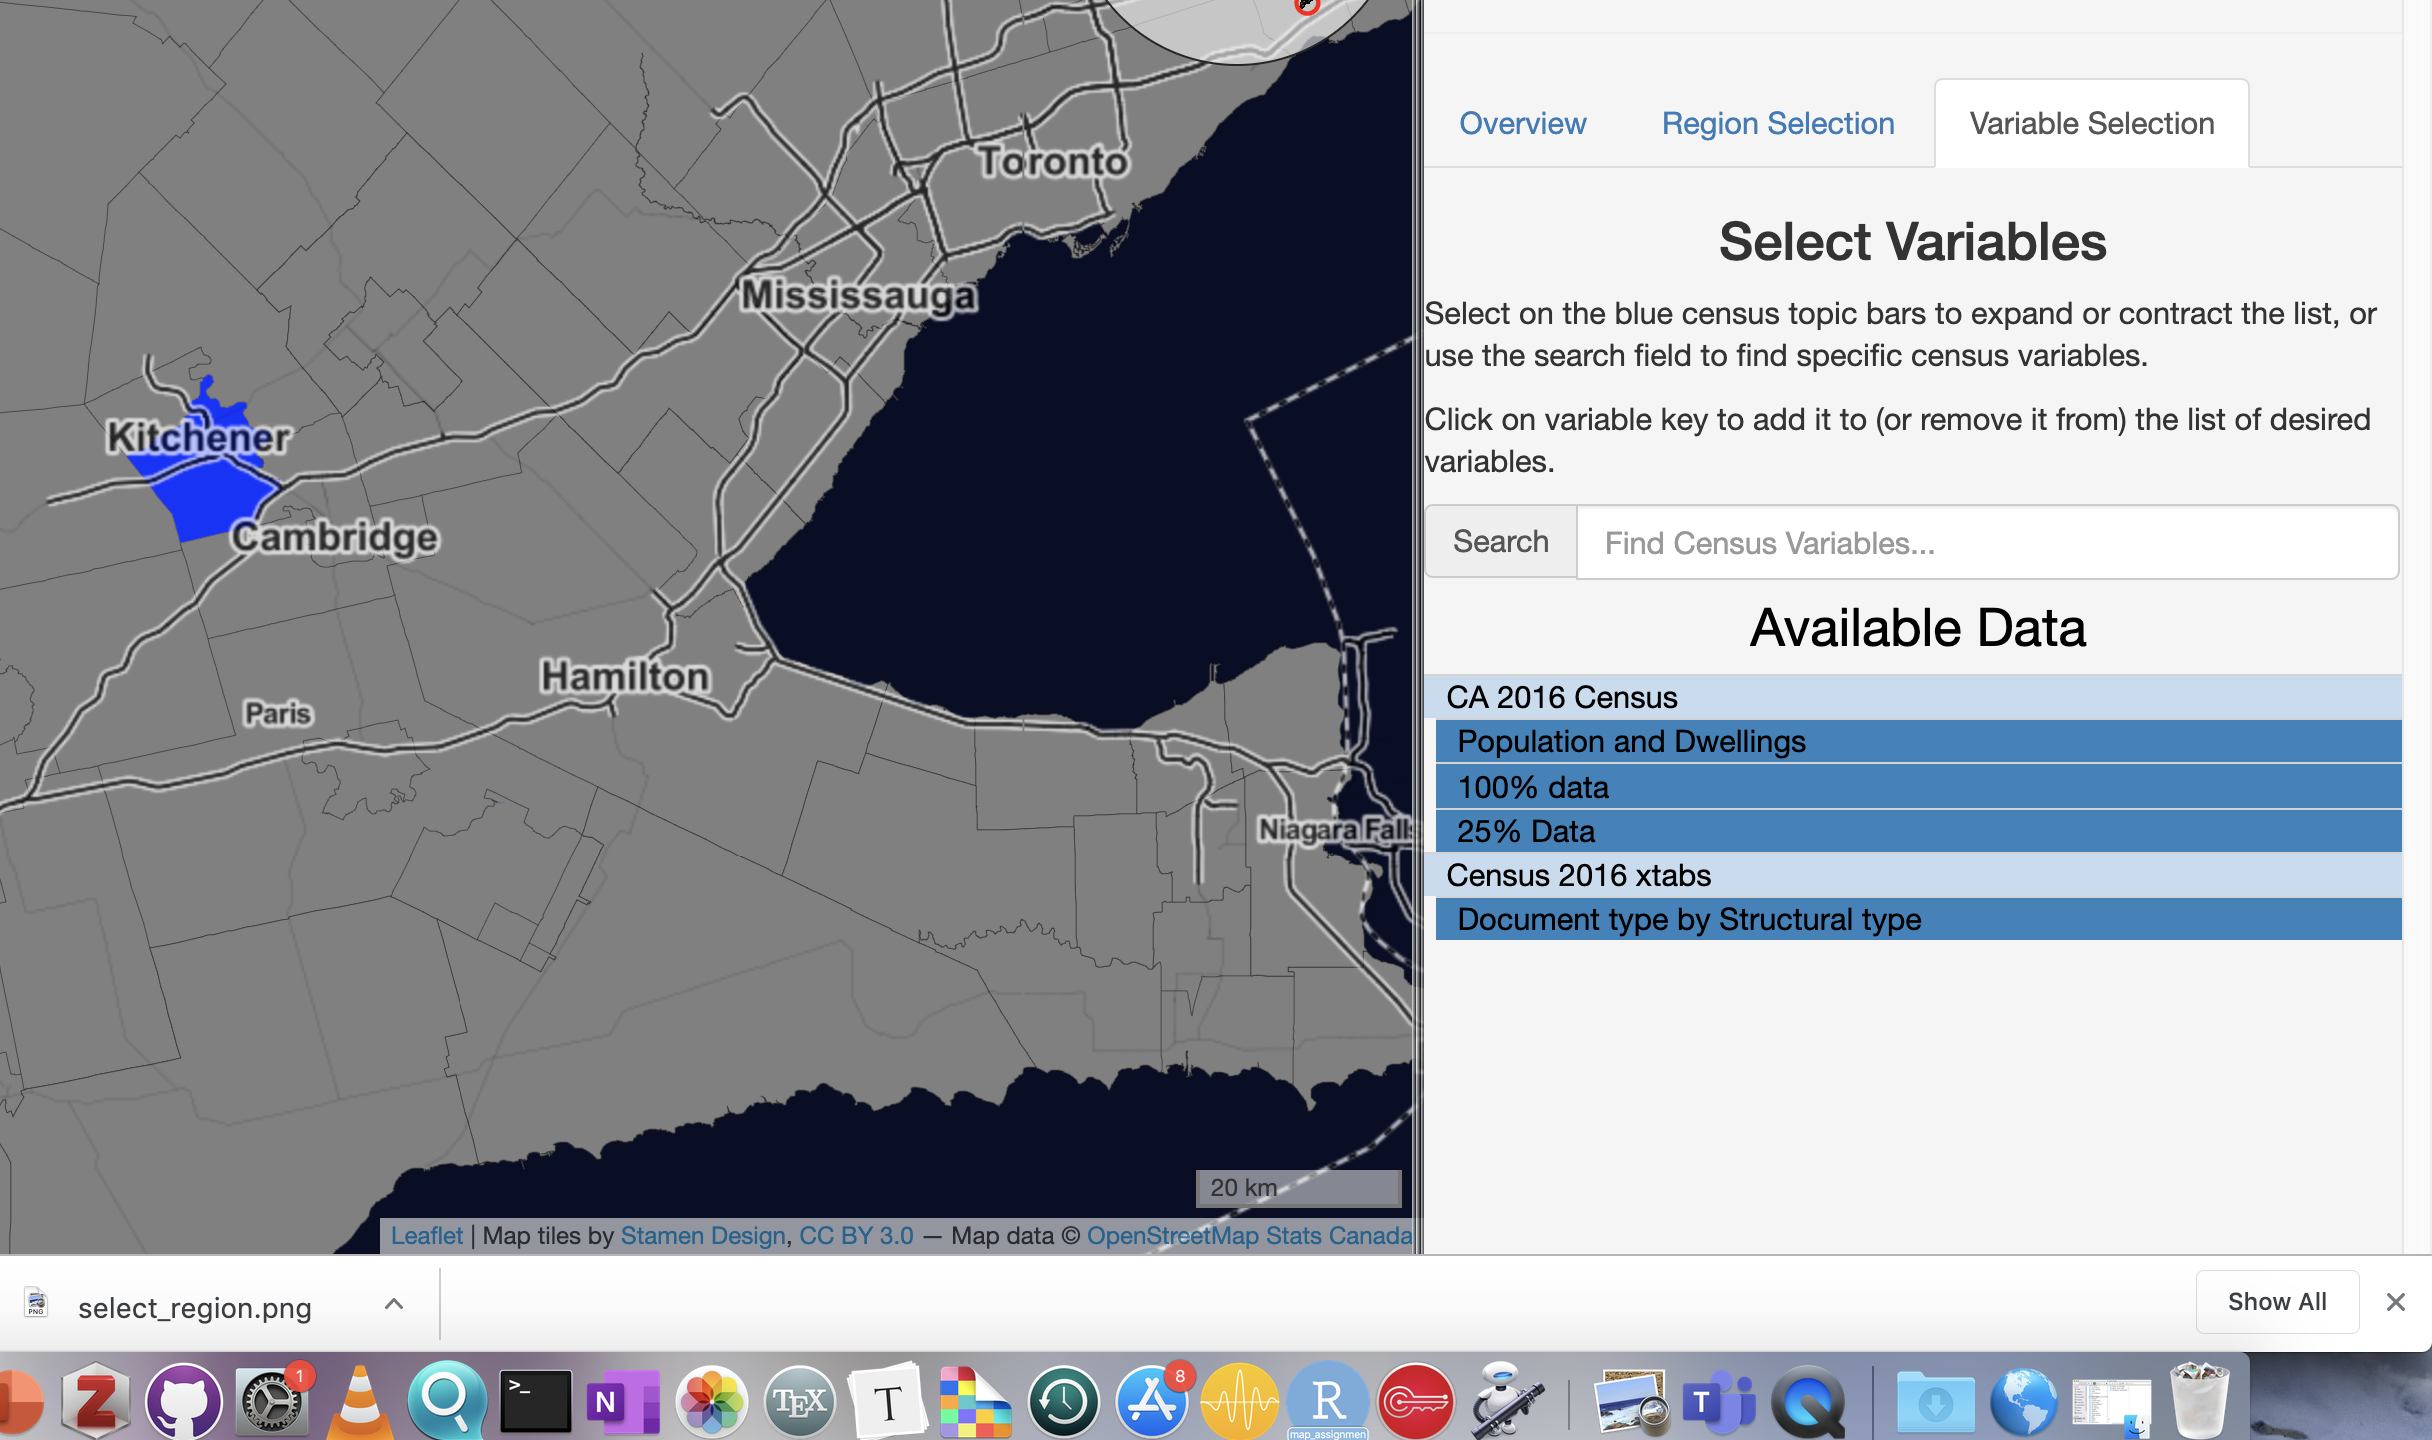
\includegraphics[width=0.5\linewidth]{images/select_kitchener_variables} \end{center}

Note that there are two categories at the top: \texttt{100\%\ Data} and
\texttt{25\%\ Data}. The difference between the two is that the first is
the results from \emph{every single household and person that filled out
the census} and the second is the results of sample drawn from the full
census (25\% of the results). So, it is a \emph{huge} sample and
extremely accurate, but it is still just a \emph{sample}.

Some variables are only released with sample data, basically out of
privacy concerns (I think).

You can search by keyword, or browse through by topics.

There are a few things to really note:

\begin{enumerate}
\def\labelenumi{\arabic{enumi}.}
\item
  Each variable appears to be summarized by sex. That is, if you want,
  you can track the results of each variable in the sense for men, women
  or total (if you do not care to differentiate by sex.)
\item
  Each variable has a code attached to it that starts with a \texttt{v}.
  e.g.~The \texttt{Total\ age} variable is \texttt{V\_CA16\_1}.
  \texttt{V} stands for \texttt{vector}, \texttt{CA16} is the 2016
  Census and \texttt{1} is just the identifier of the individual vector.
\end{enumerate}

A vector is a string of numbers that represents the variable in
question.

Now, we're not going to get that vector, because it will only tell us
the Total number of people who provided Age data to the census.

But if you click on it and you'll see that it expands into more
categories, with more vectors. Now, there is a female 0 to 14 years
vector, a male 0 to 14 years vector and a total 0 to 14 years vector.

So those three vectors will provide us with the number of females, males
and total (both sexes) 0 to 14 years old in each dissemination area in
Kitchener.

You can click on the 0 to 14 years vector as well and you see that you
get finer-grained vectors. Now you have the number of 0 to 4 year olds,
5 to 9 year olds etc, for males and females and total (both sexes.)

Click on 0 to 4 one more time and you see you get right down to the one
year category. Note: not all variables in the census will have vectors
with this level of detail.

For now, let's just select the vector that has the total number of 0 to
4 year olds. This will tell us where the toddlers live in Kitchener.
Clicking on a vector selects it, and it should appear in the text box
above the list of vectors. Clicking on it again, deselcts and clear i

Go back to the \texttt{Overview} screen and you'll see R code again. It
should look like this.

\begin{Shaded}
\begin{Highlighting}[]
\NormalTok{census\_data <{-}}\StringTok{ }\KeywordTok{get\_census}\NormalTok{(}\DataTypeTok{dataset =} \StringTok{"CA16"}\NormalTok{, }\DataTypeTok{regions =} \KeywordTok{list}\NormalTok{(}\DataTypeTok{CSD =} \StringTok{"3530013"}\NormalTok{), }\DataTypeTok{vectors =} \KeywordTok{c}\NormalTok{(}\StringTok{"v\_CA16\_4"}\NormalTok{), }
    \DataTypeTok{labels =} \StringTok{"detailed"}\NormalTok{, }\DataTypeTok{geo\_format =} \OtherTok{NA}\NormalTok{, }\DataTypeTok{level =} \StringTok{"DA"}\NormalTok{)}
\end{Highlighting}
\end{Shaded}

Notice that this is exactly the same code as above; the only difference
is that the \texttt{vectors} argument actually has something in it;
namely \texttt{v\_CA16\_}, which is the total age vector.

I'm going to modify the code a little bit. We'll call the new dataframe
\texttt{kitchener} again and remember you have to specify which
geographical file format you want.

\begin{Shaded}
\begin{Highlighting}[]
\NormalTok{kitchener2 <{-}}\StringTok{ }\KeywordTok{get\_census}\NormalTok{(}\DataTypeTok{dataset =} \StringTok{"CA16"}\NormalTok{, }\DataTypeTok{regions =} \KeywordTok{list}\NormalTok{(}\DataTypeTok{CSD =} \StringTok{"3530013"}\NormalTok{), }\DataTypeTok{vectors =} \KeywordTok{c}\NormalTok{(}\StringTok{"v\_CA16\_4"}\NormalTok{), }
    \DataTypeTok{labels =} \StringTok{"detailed"}\NormalTok{, }\DataTypeTok{geo\_format =} \StringTok{"sf"}\NormalTok{, }\DataTypeTok{level =} \StringTok{"DA"}\NormalTok{)}
\end{Highlighting}
\end{Shaded}

\begin{verbatim}
## Downloading: 3.6 kB     Downloading: 3.6 kB     Downloading: 4.5 kB     Downloading: 4.5 kB     Downloading: 4.5 kB     Downloading: 4.5 kB     Downloading: 4.5 kB     Downloading: 4.5 kB
\end{verbatim}

Now we glimpse the data again to take a look.

\begin{Shaded}
\begin{Highlighting}[]
\KeywordTok{glimpse}\NormalTok{(kitchener2)}
\end{Highlighting}
\end{Shaded}

\begin{verbatim}
## Observations: 314
## Variables: 14
## $ `Shape Area`              <dbl> 0.78200, 0.33188, 0.56447, 0.18680, 0.162...
## $ Type                      <fct> DA, DA, DA, DA, DA, DA, DA, DA, DA, DA, D...
## $ Dwellings                 <int> 230, 191, 254, 210, 199, 223, 306, 283, 1...
## $ Households                <int> 223, 168, 244, 210, 194, 217, 284, 268, 1...
## $ GeoUID                    <chr> "35300097", "35300098", "35300099", "3530...
## $ Population                <int> 588, 402, 552, 491, 425, 513, 584, 532, 4...
## $ CD_UID                    <chr> "3530", "3530", "3530", "3530", "3530", "...
## $ CSD_UID                   <chr> "3530013", "3530013", "3530013", "3530013...
## $ CT_UID                    <chr> "5410024.00", "5410024.00", "5410023.00",...
## $ CMA_UID                   <chr> "35541", "35541", "35541", "35541", "3554...
## $ geometry                  <MULTIPOLYGON [°]> MULTIPOLYGON (((-80.49342 4....
## $ `Region Name`             <fct> Kitchener, Kitchener, Kitchener, Kitchene...
## $ `Area (sq km)`            <dbl> 0.78200, 0.33188, 0.56447, 0.18680, 0.162...
## $ `v_CA16_4: 0 to 14 years` <dbl> 90, 60, 70, 70, 55, 90, 60, 65, 75, 25, 3...
\end{verbatim}

Now, we have something that looks like the same dataset, but it has 14,
rather than 11 variables. And the 14th variable
\texttt{v\_CA16\_4:\ 0\ to\ 14\ years} is the one that we really want.
It's a \texttt{dbl} variable, which is a fancy, overly complicated way
of saying that it's a number tnat can have decimal numbers.

Now we could map out where the toddlers in Kitchener live. But before we
do that, we might want to rename that ugly variable name.

We have practiced using the \texttt{rename()} command. There are two
ways to use it, oen without pipes one with. Both of these below are
equivalent.

\begin{Shaded}
\begin{Highlighting}[]
\CommentTok{\# Check the original names}
\KeywordTok{names}\NormalTok{(kitchener2)}
\end{Highlighting}
\end{Shaded}

\begin{verbatim}
##  [1] "Shape Area"              "Type"                   
##  [3] "Dwellings"               "Households"             
##  [5] "GeoUID"                  "Population"             
##  [7] "CD_UID"                  "CSD_UID"                
##  [9] "CT_UID"                  "CMA_UID"                
## [11] "geometry"                "Region Name"            
## [13] "Area (sq km)"            "v_CA16_4: 0 to 14 years"
\end{verbatim}

\begin{Shaded}
\begin{Highlighting}[]
\CommentTok{\# Option 1}
\NormalTok{kitchener3 <{-}}\StringTok{ }\KeywordTok{rename}\NormalTok{(kitchener2, }\DataTypeTok{Toddlers =} \StringTok{\textasciigrave{}}\DataTypeTok{v\_CA16\_4: 0 to 14 years}\StringTok{\textasciigrave{}}\NormalTok{)}

\CommentTok{\# Option 2 with pipes}
\NormalTok{kitchener3 <{-}}\StringTok{ }\NormalTok{kitchener2 }\OperatorTok{\%>\%}\StringTok{ }\KeywordTok{rename}\NormalTok{(}\DataTypeTok{Toddlers =} \StringTok{\textasciigrave{}}\DataTypeTok{v\_CA16\_4: 0 to 14 years}\StringTok{\textasciigrave{}}\NormalTok{)}

\CommentTok{\# Option 2a with pipes This is my favourite way because it is so logical The}
\CommentTok{\# saving part comes at the end}
\NormalTok{kitchener3 <{-}}\StringTok{ }\NormalTok{kitchener2 }\OperatorTok{\%>\%}\StringTok{ }\KeywordTok{rename}\NormalTok{(}\DataTypeTok{Toddlers =} \StringTok{\textasciigrave{}}\DataTypeTok{v\_CA16\_4: 0 to 14 years}\StringTok{\textasciigrave{}}\NormalTok{)}
\end{Highlighting}
\end{Shaded}

\begin{Shaded}
\begin{Highlighting}[]
\CommentTok{\# Check the new names}
\KeywordTok{names}\NormalTok{(kitchener3)}
\end{Highlighting}
\end{Shaded}

\begin{verbatim}
##  [1] "Shape Area"   "Type"         "Dwellings"    "Households"   "GeoUID"      
##  [6] "Population"   "CD_UID"       "CSD_UID"      "CT_UID"       "CMA_UID"     
## [11] "geometry"     "Region Name"  "Area (sq km)" "Toddlers"
\end{verbatim}

Then we can draw the map showing the number of toddlers in each
dissemination area.

\begin{Shaded}
\begin{Highlighting}[]
\KeywordTok{ggplot}\NormalTok{(kitchener3, }\KeywordTok{aes}\NormalTok{(}\DataTypeTok{geometry =}\NormalTok{ geometry, }\DataTypeTok{fill =}\NormalTok{ Toddlers)) }\OperatorTok{+}\StringTok{ }\KeywordTok{geom\_sf}\NormalTok{()}
\end{Highlighting}
\end{Shaded}

\begin{center}\includegraphics[width=0.5\linewidth]{cancensus_tutorial_files/figure-latex/toddler-map-1} \end{center}

Now, note that these are \emph{raw} numbers. If you wanted to show the
percent of the population to control for how many people live in each
dissemination area, we would have to make a percentage variable. That is
pretty easy and we have done it before in the dataset on whales earlier
in the online exercises.

\begin{Shaded}
\begin{Highlighting}[]
\CommentTok{\# check the names}
\KeywordTok{names}\NormalTok{(kitchener3)}
\end{Highlighting}
\end{Shaded}

\begin{verbatim}
##  [1] "Shape Area"   "Type"         "Dwellings"    "Households"   "GeoUID"      
##  [6] "Population"   "CD_UID"       "CSD_UID"      "CT_UID"       "CMA_UID"     
## [11] "geometry"     "Region Name"  "Area (sq km)" "Toddlers"
\end{verbatim}

Because we already have the Population variable, we can just divide the
number of Toddlers by the population and then we will get a percentage
of the total population and multiply by 100

We use the \texttt{mutate()} command to make a new variable. The
following two ways are \emph{equivalent}

\begin{Shaded}
\begin{Highlighting}[]
\CommentTok{\# Option 1 without pipes}
\NormalTok{kitchener4 <{-}}\StringTok{ }\KeywordTok{mutate}\NormalTok{(kitchener3, }\DataTypeTok{percent =}\NormalTok{ (Toddlers}\OperatorTok{/}\NormalTok{Population) }\OperatorTok{*}\StringTok{ }\DecValTok{100}\NormalTok{)}

\CommentTok{\# option 2 with pipes}
\NormalTok{kitchener4 <{-}}\StringTok{ }\NormalTok{kitchener3 }\OperatorTok{\%>\%}\StringTok{ }\KeywordTok{mutate}\NormalTok{(}\DataTypeTok{percent =}\NormalTok{ (Toddlers}\OperatorTok{/}\NormalTok{Population }\OperatorTok{*}\StringTok{ }\DecValTok{100}\NormalTok{))}

\CommentTok{\# option 2a with pipes}

\NormalTok{kitchener4 <{-}}\StringTok{ }\NormalTok{kitchener3 }\OperatorTok{\%>\%}\StringTok{ }\KeywordTok{mutate}\NormalTok{(}\DataTypeTok{percent =}\NormalTok{ (Toddlers}\OperatorTok{/}\NormalTok{Population }\OperatorTok{*}\StringTok{ }\DecValTok{100}\NormalTok{))}
\end{Highlighting}
\end{Shaded}

Then we can redraw using the exact same code. Note that our
\texttt{fill} variable is different now though, because we are not
filling based on the number of Toddlers, but the percent variable that
we created above.

\begin{Shaded}
\begin{Highlighting}[]
\KeywordTok{ggplot}\NormalTok{(kitchener4, }\KeywordTok{aes}\NormalTok{(}\DataTypeTok{geometry =}\NormalTok{ geometry, }\DataTypeTok{fill =}\NormalTok{ percent)) }\OperatorTok{+}\StringTok{ }\KeywordTok{geom\_sf}\NormalTok{()}
\end{Highlighting}
\end{Shaded}

\begin{center}\includegraphics[width=0.5\linewidth]{cancensus_tutorial_files/figure-latex/plot-percent-1} \end{center}

\hypertarget{how-do-we-add-in-a-third-variable.}{%
\subsection{How do we add in a third
variable.}\label{how-do-we-add-in-a-third-variable.}}

Let's just say that we want to break out the toddlers by sex. It's
important to remember: Statistics Canada is not providing us with the
individual level data from the census. They are aggregating it for us.
What this means is that we cannot do a lot of crosstabulations by
different variables.

For example, we could not show the distribution of toddlers of different
ethnicities, for example unless Statistics Canada provides us with a
table that has those two variables already combined.

The only variable that is almost always crosstabbed is sex. So we can
always go back to the 0 to 4 years category and select the female and
the male vectors.

The R code looks like this. Note this is the exact code to download the
Kitchener data as above. I've just changed the vector numbers and saved
this in \texttt{kitchener5}

\begin{Shaded}
\begin{Highlighting}[]
\NormalTok{kitchener5 <{-}}\StringTok{ }\KeywordTok{get\_census}\NormalTok{(}\DataTypeTok{dataset =} \StringTok{"CA16"}\NormalTok{, }\DataTypeTok{regions =} \KeywordTok{list}\NormalTok{(}\DataTypeTok{CSD =} \StringTok{"3530013"}\NormalTok{), }\DataTypeTok{vectors =} \KeywordTok{c}\NormalTok{(}\StringTok{"v\_CA16\_9"}\NormalTok{, }
    \StringTok{"v\_CA16\_8"}\NormalTok{), }\DataTypeTok{labels =} \StringTok{"detailed"}\NormalTok{, }\DataTypeTok{geo\_format =} \StringTok{"sf"}\NormalTok{, }\DataTypeTok{level =} \StringTok{"DA"}\NormalTok{)}
\end{Highlighting}
\end{Shaded}

Note, how we're getting two new vectors.

\begin{Shaded}
\begin{Highlighting}[]
\KeywordTok{glimpse}\NormalTok{(kitchener5)}
\end{Highlighting}
\end{Shaded}

Observations: 314 Variables: 15 \$ \texttt{Shape\ Area} 0.78200,
0.33188, 0.56447, 0.18680, 0.1620\ldots{} \$ Type DA, DA, DA, DA, DA,
DA, DA, DA, DA, DA, DA\ldots{} \$ Dwellings 230, 191, 254, 210, 199,
223, 306, 283, 18\ldots{} \$ Households 223, 168, 244, 210, 194, 217,
284, 268, 18\ldots{} \$ GeoUID ``35300097'', ``35300098'', ``35300099'',
``35300\ldots{} \$ Population 588, 402, 552, 491, 425, 513, 584, 532,
45\ldots{} \$ CD\_UID
''3530``,''3530``,''3530``,''3530``,''3530``,''3\ldots{} \$ CSD\_UID
``3530013'', ``3530013'', ``3530013'', ``3530013''\ldots{} \$ CT\_UID
``5410024.00'', ``5410024.00'', ``5410023.00'', \ldots{} \$ CMA\_UID
``35541'', ``35541'', ``35541'', ``35541'', "35541\ldots{} \$ geometry
\textless MULTIPOLYGON {[}°{]}\textgreater{} MULTIPOLYGON (((-80.49342
4\ldots.. \$ \texttt{Region\ Name} Kitchener, Kitchener, Kitchener,
Kitchener\ldots{} \$ \texttt{Area\ (sq\ km)} 0.78200, 0.33188, 0.56447,
0.18680, 0.1620\ldots{} \$ \texttt{v\_CA16\_9:\ 0\ to\ 4\ years} 10, 10,
20, 10, 10, 10, 15, 20, 15, 10, 5,\ldots{} \$
\texttt{v\_CA16\_8:\ 0\ to\ 4\ years} 15, 10, 10, 15, 15, 15, 10, 15,
10, 10, 10\ldots{} Those variable names are ugly so we should rename
them again. If we go back to the website, we know that vector
\texttt{v\_CA16\_9} is females and vector \texttt{v\_CA16\_8} is males.

And remember, we can use the \texttt{rename} command based on position
as well as by name. This would work on the \texttt{rename()}commands
above, as well, you just need to identify what the variable names are
that you need to rename.

\begin{Shaded}
\begin{Highlighting}[]
\CommentTok{\# check names}
\KeywordTok{names}\NormalTok{(kitchener5)}
\end{Highlighting}
\end{Shaded}

\begin{verbatim}
##  [1] "Shape Area"             "Type"                   "Dwellings"             
##  [4] "Households"             "GeoUID"                 "Population"            
##  [7] "CD_UID"                 "CSD_UID"                "CT_UID"                
## [10] "CMA_UID"                "geometry"               "Region Name"           
## [13] "Area (sq km)"           "v_CA16_9: 0 to 4 years" "v_CA16_8: 0 to 4 years"
\end{verbatim}

We are going to change the names of variables 14 and 15.

\begin{Shaded}
\begin{Highlighting}[]
\CommentTok{\# option 1}
\NormalTok{kitchener6 <{-}}\StringTok{ }\KeywordTok{rename}\NormalTok{(kitchener5, }\DataTypeTok{Females =} \DecValTok{14}\NormalTok{, }\DataTypeTok{Males =} \DecValTok{15}\NormalTok{)}

\CommentTok{\# option 2 with pipes}
\NormalTok{kitchener6 <{-}}\StringTok{ }\NormalTok{kitchener5 }\OperatorTok{\%>\%}\StringTok{ }\KeywordTok{rename}\NormalTok{(}\DataTypeTok{Females =} \DecValTok{14}\NormalTok{, }\DataTypeTok{Males =} \DecValTok{15}\NormalTok{)}

\CommentTok{\# option 2a}
\NormalTok{kitchener6 <{-}}\StringTok{ }\NormalTok{kitchener5 }\OperatorTok{\%>\%}\StringTok{ }\KeywordTok{rename}\NormalTok{(}\DataTypeTok{Females =} \DecValTok{14}\NormalTok{, }\DataTypeTok{Males =} \DecValTok{15}\NormalTok{)}
\end{Highlighting}
\end{Shaded}

\begin{Shaded}
\begin{Highlighting}[]
\CommentTok{\# rechecknames}
\KeywordTok{names}\NormalTok{(kitchener6)}
\end{Highlighting}
\end{Shaded}

\begin{verbatim}
##  [1] "Shape Area"   "Type"         "Dwellings"    "Households"   "GeoUID"      
##  [6] "Population"   "CD_UID"       "CSD_UID"      "CT_UID"       "CMA_UID"     
## [11] "geometry"     "Region Name"  "Area (sq km)" "Females"      "Males"
\end{verbatim}

Now the othe problem is that this is not tidy data. There are two
different y-variables (\texttt{Females} and \texttt{Males}.)

Using the \texttt{gather()} command, we say what is the new \texttt{key}
variable going to be called (i.e.~\texttt{Sex}, the new value variable
\texttt{n} and which variables get gathered).

\begin{Shaded}
\begin{Highlighting}[]
\CommentTok{\# option 1}
\NormalTok{kitchener7 <{-}}\StringTok{ }\KeywordTok{gather}\NormalTok{(kitchener6, Sex, n, Females, Males)}

\CommentTok{\# Optino 2 you can do it with pipes.}
\NormalTok{kitchener7 <{-}}\StringTok{ }\NormalTok{kitchener6 }\OperatorTok{\%>\%}\StringTok{ }\KeywordTok{gather}\NormalTok{(Sex, n, Females, Males)}

\CommentTok{\# option2a}
\NormalTok{kitchener7 <{-}}\StringTok{ }\NormalTok{kitchener6 }\OperatorTok{\%>\%}\StringTok{ }\KeywordTok{gather}\NormalTok{(Sex, n, Females, Males)}
\end{Highlighting}
\end{Shaded}

\begin{Shaded}
\begin{Highlighting}[]
\KeywordTok{glimpse}\NormalTok{(kitchener7)}
\end{Highlighting}
\end{Shaded}

\begin{verbatim}
## Observations: 628
## Variables: 15
## $ `Shape Area`   <dbl> 0.78200, 0.33188, 0.56447, 0.18680, 0.16206, 0.15935...
## $ Type           <fct> DA, DA, DA, DA, DA, DA, DA, DA, DA, DA, DA, DA, DA, ...
## $ Dwellings      <int> 230, 191, 254, 210, 199, 223, 306, 283, 185, 360, 22...
## $ Households     <int> 223, 168, 244, 210, 194, 217, 284, 268, 185, 357, 21...
## $ GeoUID         <chr> "35300097", "35300098", "35300099", "35300100", "353...
## $ Population     <int> 588, 402, 552, 491, 425, 513, 584, 532, 459, 530, 37...
## $ CD_UID         <chr> "3530", "3530", "3530", "3530", "3530", "3530", "353...
## $ CSD_UID        <chr> "3530013", "3530013", "3530013", "3530013", "3530013...
## $ CT_UID         <chr> "5410024.00", "5410024.00", "5410023.00", "5410023.0...
## $ CMA_UID        <chr> "35541", "35541", "35541", "35541", "35541", "35541"...
## $ geometry       <MULTIPOLYGON [°]> MULTIPOLYGON (((-80.49342 4..., MULTIPO...
## $ `Region Name`  <fct> Kitchener, Kitchener, Kitchener, Kitchener, Kitchene...
## $ `Area (sq km)` <dbl> 0.78200, 0.33188, 0.56447, 0.18680, 0.16206, 0.15935...
## $ Sex            <chr> "Females", "Females", "Females", "Females", "Females...
## $ n              <dbl> 10, 10, 20, 10, 10, 10, 15, 20, 15, 10, 5, 5, 10, 15...
\end{verbatim}

Now we could draw the map and facet on sex. Note now we have named the
variable that has the actual number of toddlers to be \texttt{n}.

\begin{Shaded}
\begin{Highlighting}[]
\KeywordTok{ggplot}\NormalTok{(kitchener7, }\KeywordTok{aes}\NormalTok{(}\DataTypeTok{geometry =}\NormalTok{ geometry, }\DataTypeTok{fill =}\NormalTok{ n)) }\OperatorTok{+}\StringTok{ }\KeywordTok{geom\_sf}\NormalTok{() }\OperatorTok{+}\StringTok{ }\KeywordTok{facet\_wrap}\NormalTok{(}\OperatorTok{\textasciitilde{}}\NormalTok{Sex)}
\end{Highlighting}
\end{Shaded}

\begin{center}\includegraphics[width=0.5\linewidth]{cancensus_tutorial_files/figure-latex/facet-1} \end{center}

\end{document}
